\documentclass{tufte-book}

% \usepackage{palatino, fullpage}
% \addbibresource{lib/bib.bib}
% \newcommand\citet[1]{\textcite{#1}}
\newcommand\jl{{\color{red}JL: }}
\newcommand\sh[1]{{\color{red}SH: #1}}


\usepackage{amsmath,amsthm}
\usepackage{tikz,tikz-cd,relsize,hyperref}
\usepackage[nameinlink,capitalise]{cleveref} \usepackage{enumitem}
\usepackage{mathtools,subcaption}
\usepackage{amsmath,amssymb,stmaryrd,mathpartir,listings,xcolor}
\usepackage[utf8]{inputenc} % for hiragana yo
\usepackage{mdframed}

\usetikzlibrary{positioning,arrows}

\mdfdefinestyle{theoremstyle}{%
  linecolor=black,linewidth=1pt,%
  frametitlerule=true,%
  frametitlebackgroundcolor=gray!20,
  innertopmargin=\topskip,
}
\mdtheorem[style=theoremstyle]{definition}{Definition}

\definecolor{codegreen}{rgb}{0,0.6,0}
\definecolor{codegray}{rgb}{0.5,0.5,0.5}
\definecolor{codepurple}{rgb}{0.58,0,0.82}
\definecolor{backcolour}{rgb}{0.95,0.95,0.92}

\lstdefinestyle{mystyle}{
    backgroundcolor=\color{backcolour},   
    commentstyle=\color{codegreen},
    keywordstyle=\color{magenta},
    numberstyle=\tiny\color{codegray},
    stringstyle=\color{codepurple},
    basicstyle=\ttfamily\footnotesize,
    breakatwhitespace=false,         
    breaklines=true,                 
    captionpos=b,                    
    keepspaces=true,                 
    numbers=left,                    
    numbersep=5pt,                  
    showspaces=false,                
    showstringspaces=false,
    showtabs=false,                  
    tabsize=2
}

\lstset{style=mystyle}


% This order is important: \newtheorem needs to be after importing \cleveref
% https://stackoverflow.com/questions/6499504/cleveref-fails-for-theorem-environments-sharing-the-same-counter
\theoremstyle{definition}
\newtheorem{theorem}{Theorem}[section]
\newtheorem{corollary}[theorem]{Corollary}
\newtheorem{lemma}[theorem]{Lemma}
\newtheorem{hope}[theorem]{Hope}
\newtheorem{belief}[theorem]{Belief}
\newtheorem{construction}[theorem]{Construction}
\newtheorem{intuition}[theorem]{Intuition}
% \newtheorem{definition}[theorem]{Definition}
\newtheorem{notation}[theorem]{Notation}
\newtheorem{example}[theorem]{Example}
\newtheorem{warning}[theorem]{Warning}
\newtheorem{claim}[theorem]{Claim}
\newtheorem{procedure}[theorem]{Procedure}
\newtheorem{note}[theorem]{Note}
\newtheorem{question}[theorem]{Question}
\newtheorem{fact}[theorem]{Fact}
\newtheorem{assumption}[theorem]{{\color{red}Assumption}}
\newtheorem{metatheorem}[theorem]{Metatheorem}
\newtheorem{proposition}[theorem]{Proposition}
\newtheorem{remark}[theorem]{Remark}
\newtheorem{problem}{Problem}
\newtheorem{problem-part}{Part}[problem]
\newenvironment{answer}{\renewcommand{\proofname}{Answer}\begin{proof}}{\end{proof}}
\crefname{theorem}{Theorem}{Theorems}
\crefname{construction}{Construction}{Constructions}
\crefname{corollary}{Corollary}{Corollaries}
\crefname{lemma}{Lemma}{Lemmas}
\crefname{hope}{Hope}{Hopes}
\crefname{belief}{Belief}{Beliefs}
\crefname{construction}{Construction}{Constructions}
\crefname{intuition}{Intuition}{Intuitions}
\crefname{definition}{Definition}{Definitions}
\crefname{notation}{Notation}{Notations}
\crefname{example}{Example}{Examples}
\crefname{warning}{Warning}{Warnings}
\crefname{claim}{Claim}{Claims}
\crefname{procedure}{Procedure}{Procedures}
\crefname{note}{Note}{Notes}
\crefname{question}{Question}{Questions}
\crefname{fact}{Fact}{Facts}
\crefname{assumption}{Assumption}{Assumptions}
\crefname{metatheorem}{Metatheorem}{Metatheorems}
\crefname{proposition}{Proposition}{Propositions}
\crefname{metatheorem}{Metatheorem}{Metatheorems}
\crefname{problem}{Problem}{Problems}
\crefname{problem-part}{Part}{Parts}

\DeclareFontFamily{U}{min}{}
\DeclareFontShape{U}{min}{m}{n}{<-> udmj30}{}
\newcommand\yo{\!\text{\usefont{U}{min}{m}{n}\symbol{'207}}\!}

\newcommand\subtext[1]{{\color{lightgray}#1}}

\newcommand\Set{\mathsf{Set}}
\newcommand\FinSet{\mathsf{FinSet}}
\newcommand\Cat{\mathsf{Cat}}
\newcommand\Vect{\mathsf{Vect}}
\newcommand\Group{\mathsf{Group}}
\newcommand\ofty{\,{:}\,}
\newcommand\bool{\mathrm{bool}}
\newcommand\true{\mathrm{true}}
\newcommand\false{\mathrm{false}}
\newcommand\colim{\operatorname{colim}}
\newcommand\copi{\text{\rotatebox[origin=c]{180}{$\pi$}}}
\newcommand\adjunct{\mathop{\text{\reflectbox{$\rightleftarrows$}}}}
\newcommand\img{\operatorname{im}}
\newcommand\Sh{\operatorname{Sh}}
\newcommand\psh{\operatorname{PSh}}
\newcommand\Aut{\operatorname{Aut}}
\newcommand{\ama}{\operatorname{\mathsf{amalg}}}
\newcommand{\dom}{\operatorname{\mathsf{dom}}}
\newcommand{\cod}{\operatorname{\mathsf{cod}}}
\newcommand{\idt}{\mathsf{id}}
\newcommand\todo{{\color{red}\bf todo}}
\newcommand\Sub{\operatorname{Sub}}
\newcommand\Hom{\operatorname{Hom}}
\newcommand\id{\operatorname{id}}
\newcommand\dnclose{\operatorname{\downarrow}}
\newcommand\genelt[2]{\mathsf{Elt}_{#2}(#1)}
\newcommand\calA{\mathcal A}
\newcommand\calB{\mathcal B}
\newcommand\calC{\mathcal C}
\newcommand\calD{\mathcal D}
\newcommand\calE{\mathcal E}
\newcommand\calF{\mathcal F}
\newcommand\calG{\mathcal G}
\newcommand\calH{\mathcal H}
\newcommand\calI{\mathcal I}
\newcommand\calJ{\mathcal J}
\newcommand\calK{\mathcal K}
\newcommand\calL{\mathcal L}
\newcommand\calM{\mathcal M}
\newcommand\calN{\mathcal N}
\newcommand\calO{\mathcal O}
\newcommand\calP{\mathcal P}
\newcommand\calQ{\mathcal Q}
\newcommand\calR{\mathcal R}
\newcommand\calS{\mathcal S}
\newcommand\calT{\mathcal T}
\newcommand\calU{\mathcal U}
\newcommand\calV{\mathcal V}
\newcommand\mor[1]{\xrightarrow{#1}}
\newcommand\llbr[1]{\left\llbracket #1\right\rrbracket}
\newcommand\ite[3]{\mathrm{if}~#1~\mathrm{then}~#2~\mathrm{else}~#3}
\newcommand\R{\mathbb R}
\newcommand\N{\mathbb N}
\newcommand\Q{\mathbb Q}
\newcommand\Z{\mathbb Z}
\newcommand\Ber{\operatorname{Ber}}
\newcommand\Ob{\operatorname{Ob}}
\newcommand\angled[1]{\langle #1\rangle}
\newcommand\frakA{\mathfrak A}
\newcommand\frakB{\mathfrak B}
\newcommand\frakC{\mathfrak C}
\newcommand\frakD{\mathfrak D}
\newcommand\frakE{\mathfrak E}
\newcommand\frakF{\mathfrak F}
\newcommand\frakG{\mathfrak G}
\newcommand\frakH{\mathfrak H}
\newcommand\frakM{\mathfrak M}
\newcommand\frakN{\mathfrak N}
\newcommand\frakO{\mathfrak O}
\newcommand\frakP{\mathfrak P}
\newcommand\frakQ{\mathfrak Q}
\newcommand\frakU{\mathfrak U}
\newcommand\frakV{\mathfrak V}
\newcommand\stepsto{\rightarrow}

\newcommand\plkwcolor[1]{{\color{blue}#1}}
\newcommand\pllitcolor[1]{{\color{teal}#1}}
\newcommand\plfont[1]{\mathsf{#1}}
\newcommand\dbracket[1]{\left\llbracket #1 \right\rrbracket}
\newcommand\sem[1]{{\color{blue} #1}}
\newcommand\plkw[1]{\plfont{\plkwcolor{#1}}}
\newcommand\pllit[1]{\mathsf{\pllitcolor{#1}}}
\newcommand\pllet[3]{\plkw{let}~#1~\plkw{be}~#2~\plkw{in}~#3}
\newcommand\plret[1]{\plkw{ret}~#1}
\newcommand\plproj[2]{\plkw{proj}_{\plkwcolor{#1}}~#2}
\newcommand\plinj[2]{\plkw{inj}_{\plkwcolor{#1}}~#2}

\newcommand\ctxemp{\mathsmaller{\mathsmaller{\bullet}}}

\newcommand\plUnit{\plkw{Unit}}
\newcommand\plunit{{\plkwcolor{\angled{}}}}

\newcommand\pltimes{\mathbin{\plkwcolor\times}}
\newcommand\plpair[2]{\plkwcolor{\angled{{\normalcolor #1\plkwcolor{,}\, #2}}}}
\newcommand\plfst[1]{\plkw{fst}\,#1}
\newcommand\plsnd[1]{\plkw{snd}\,#1}
\newcommand\plflip[0]{\plkw{flip}}
\newcommand\pltrue[0]{\plkw{true}}
\newcommand\plfalse[0]{\plkw{false}}
\newcommand\plBool[0]{\plkw{Bool}}

\newcommand\plto{\mathbin{\plkwcolor\to}}
\newcommand\pllam[2]{\plkwcolor{\lambda}\,#1\plkwcolor{.}\,#2}
\newcommand\plapp[2]{#1\,#2}

\newcommand\plVoid{\plkw{Void}}
\newcommand\plunreachable[1]{\plkw{unreachable}\,#1}

\newcommand\plplus{\mathbin{\plkwcolor+}}
\newcommand\plinl[1]{\plkw{inl}\,#1}
\newcommand\plinr[1]{\plkw{inr}\,#1}
\newcommand\plcase[5]
{\plkw{case}\plkwcolor{(}#1\plkwcolor{,}~
  #2\plkwcolor{.}\,#3\plkwcolor{,}~
  #4\plkwcolor{.}\,#5)}

% https://tikzcd.yichuanshen.de/#N4Igdg9gJgpgziAXAbVABwnAlgFyxMJZABgBpiBdUkANwEMAbAVxiRAZAF9T1Nd9CKMgEYqtRizYMA5FzEwoAc3hFQAMwBOEALZIyIHBCTDq9Zq0Qg1IagzoAjGAwAKfPATYasigBY45nEA
% 1
% |
% | 2
% v
% 3
\newcommand\vertarrow[3]{
  \begin{tikzcd}[ampersand replacement=\&]
    {#1} \arrow[d, "{#2}"'] \\
    {#3}               
  \end{tikzcd}
}

%      2
%   1 --> 3
% 4 |     | 5
%   v     v
%   6 --> 8
%      7
\newcommand\commsquare[8]{
\begin{tikzcd}[ampersand replacement=\&]
{#1} \arrow[d, "{#4}"'] \arrow[r, "{#2}"] \& {#3} \arrow[d, "{#5}"] \\
{#6} \arrow[r, "{#7}"']                \& {#8}
\end{tikzcd}
}

%      2
%   1 --> 3
% 4 | _|  | 5
%   v     v
%   6 --> 8
%      7
\newcommand\pullback[8]{
\begin{tikzcd}[ampersand replacement=\&]
{#1} \arrow[d, "{#4}"'] \arrow[r, "{#2}"]
\arrow[dr, phantom, "\lrcorner", very near start]
\& {#3} \arrow[d, "{#5}"] \\
{#6} \arrow[r, "{#7}"'] \& {#8}
\end{tikzcd}
}

% takes the arguments for \pullback first, and then takes arguments for the cone, then mediating map
\newcommand\pullbackump[3]{%
  \def\tempa{#1}%
  \def\tempb{#2}%
  \def\tempc{#3}%
  \pullbackumprest
}
\newcommand\pullbackumprest[9]{
% https://tikzcd.yichuanshen.de/#N4Igdg9gJgpgziAXAbVABwnAlgFyxMJZARgBpiBdUkANwEMAbAVxiRDpAF9T1Nd9CKAEzkqtRizYAjLjxAZseAkTJCx9Zq0QgAxrN6KBREWuobJ2qPvl8lg5AAZSD9RK0hWnMTCgBzeESgAGYAThAAtkgALNQ4EEgiIFIwYFaIALQAzE7immwAFiDUDHTJDAAKtkbaIVi++TjWoRHRsfGIZEkpadlmbmwA1k1hkYg5cUid5u5oQcMtHW1ImX152r7zo4kTiCu5FiBzxaUwFVXKNXUNm0jj7YnTbGgbx2WVhhcgtfWN3MEjrRAOxyJTe50EXyujVWByYXAonCAA
\begin{tikzcd}[ampersand replacement=\&]
  #6 \arrow[rdd, "#7"', bend right] \arrow[rrd, "#8", bend left] \arrow[rd, "#9"'] \&                                    \&                  \\
     \& \tempa \arrow[r, "\tempb"] \arrow[d, "#1"'] 
        \arrow[dr, phantom, "\lrcorner", very near start]
     \& \tempc \arrow[d, "#2"] \\
     \& #3 \arrow[r, "#4"']                  \& #5               
  \end{tikzcd}
}

%    2     4
% 1 --> 3 --> 6
%         -->
%          5 
\newcommand\weakequalizer[6]{
  \begin{tikzcd}[ampersand replacement=\&]
      #1 \arrow[r, "#2"'] 
      \& #3 \arrow[r, "#5"', shift right=1] \arrow[r, "#4", shift left=1]
      \& #6
  \end{tikzcd}
}

%    2     4
% 1 --> 3 --> 6
%         -->
%          5 
% hookrightarrow on 2
\newcommand\equalizer[6]{
  \begin{tikzcd}[ampersand replacement=\&]
      #1 \arrow[r, "#2"', hook] 
      \& #3 \arrow[r, "#5"', shift right=1] \arrow[r, "#4", shift left=1]
      \& #6
  \end{tikzcd}
}

%    2     5
% 1 --> 4 --> 6
%   --> 
%    3  
\newcommand\weakcoequalizer[6]{
  \begin{tikzcd}[ampersand replacement=\&]
      #1 \arrow[r, "#3"', shift right=1] \arrow[r, "#2", shift left=1]
      \& #4 \arrow[r, "#5"'] 
      \& #6
  \end{tikzcd}
}

%    2         4
% 1 --> 3 ----------> 6
%         ---------->
%              5
\newcommand\longequalizer[6]{
  \begin{tikzcd}[ampersand replacement=\&]
      #1 \arrow[r, "#2"', hook] 
      \& #3 \arrow[rr, "#5"', shift right=1] \arrow[rr, "#4", shift left=1]
      \& {} \& #6
  \end{tikzcd}
}

%    2
% 1 <-- 4
%   -->
%    3
\newcommand\adjunction[4]{
  {#1}~~\underset{\mathlarger{\underset {#3}\longrightarrow}}{\overset{\mathlarger{\overset {#2}\longleftarrow}}{\mathsmaller{\mathsmaller\bot}}}~~{#4}
}

%    2
% 1 ---> 3
%   \   /
%  4 \ / 5     (diagonal arrow on the right dashed)
%     6
\newcommand\uniqext[6]{
  \begin{tikzcd}[ampersand replacement = \&]
  #1 \arrow[rd, "#4"'] \arrow[rr, "#2"] \&   \& #3 \arrow[ld, "#5", dashed] \\
  \& #6 \&
  \end{tikzcd}
}

%   2      4
% 1 --> 3 --> 5
% |     |     |
% |6    |7    |8
% v     v     v
% 9 --> 11 -> 13
%   10     12
%
% https://tikzcd.yichuanshen.de/#N4Igdg9gJgpgziAXAbVABwnAlgFyxMJZABgBpiBdUkANwEMAbAVxiRDpAF9T1Nd9CKAIzkqtRizYAjLjxAZseAkQBMo6vWatEIAMazeigUTJCxmyTqgH5fJYOQizGidpCtuh-spRrn4rTYAMy4xGCgAc3giUCCAJwgAWyQyEBwIJBEAyxAAMRt4pMzqdKQ1bLcAcQKE5MRU0sQAZhdAnQAJGqLELMaAFlacgEkuuvLGgFZBtwApUaQWtIzEAYq2AGkQagY6KRgGAAU7Yx04rAiACxx5lZLlqbWdABktkB29w+OfEDPL684KJwgA
\newcommand\commrect[6]{%
  \def\tempa{#1}%
  \def\tempb{#2}%
  \def\tempc{#3}%
  \def\tempd{#4}%
  \def\tempe{#5}%
  \def\tempf{#6}%
  \commrectrest
}
\newcommand\commrectrest[7]{%
\begin{tikzcd}[ampersand replacement = \&]
\tempa \arrow[r, "\tempb"] \arrow[d, "\tempf"] \& \tempc \arrow[r, "\tempd"] \arrow[d, "#1"] \& \tempe \arrow[d, "#2"] \\
#3 \arrow[r, "#4"']               \& #5 \arrow[r, "#6"']               \& #7
\end{tikzcd}
}

%     2
%   ---->    5
% 1       4 --->> 6
%   ---->
%     3
\newcommand\coequalizer[6]{
% https://tikzcd.yichuanshen.de/#N4Igdg9gJgpgziAXAbVABwnAlgFyxMJZABgBpiBdUkANwEMAbAVxiRAGIBGEAX1PUy58hFJ3JVajFm3YAWXvxAZseAkQBM46vWatEHAGy8JMKAHN4RUADMAThAC2SMiBwQkYkHAAWWazg9tKT0OAGYQagY6ACMYBgAFQVUREFssM28Avht7J0QXN0CvX38kAFpPHWl9dnUFHMciwsRNSV0ZAFYIkG8YOig2HAB3CF7+hB4KHiA
\begin{tikzcd}[ampersand replacement=\&]
  {#1} \arrow[r, "{#3}"', shift right] \arrow[r, "{#2}", shift left] \& {#4} \arrow[r, "{#5}", two heads] \& {#6}
  \end{tikzcd}
}

%       2
%  1  ---->>  3
%  |          |
% 4|          |5
%  v          v
%  6 hook---> 8
%        7
\newcommand\strongepiunfilled[8]{
% https://tikzcd.yichuanshen.de/#N4Igdg9gJgpgziAXAbVABwnAlgFyxMJZABgBpiBdUkANwEMAbAVxiRAGIBGEAX1PUy58hFJ3JVajFm3YBmXvxAZseAkTKcJ9Zq0QcAbAoErhRMZurbpe9gA5eEmFADm8IqABmAJwgBbJGQgOBBIYpI6MgBMINQAFjB0UGw4AO4Q8YkIfJ4+-oiBwUiRllK6HAAsMSAMdABGMAwACoKqIiBeWM6xOEYg3n6h1IWIsiURNgCsvf15xUEhI0N0WAxssRAQANZVVmXsAOxVNfVNLaZ6HV09PBQ8QA
\begin{tikzcd}[ampersand replacement=\&]
  {#1} \arrow[r, "{#2}", two heads] \arrow[d, "{#4}"'] \& {#3} \arrow[d, "{#5}"] \\
  {#6} \arrow[r, "{#7}"', hook]                      \& {#8}                
  \end{tikzcd}
}

%       2
%  1  ---->>   3
%  |     /     |
% 4|  9/dashed |5
%  v v         v
%  6 hook---> 8
%        7
\newcommand\strongepi[9]{
% https://tikzcd.yichuanshen.de/#N4Igdg9gJgpgziAXAbVABwnAlgFyxMJZABgBpiBdUkANwEMAbAVxiRAGIBGEAX1PUy58hFJ3JVajFm3YBmXvxAZseAkTKcJ9Zq0QcAbAoErhRMZurbpe9gA5eEmFADm8IqABmAJwgBbJGQgOBBIYpI6MgBMINQAFjB0UGw4AO4Q8YkIfJ4+-oiBwUiRllK6HAAsMSAMdABGMAwACoKqIiBeWM6xOEYg3n6h1IWIsiURNgCsvf15xUEhI0N0WAxssRAQANZVVmXsAOxVNfVNLaZ6HV092X25g-NFY9YcAJxHWGBlUHRw8Uk8FB4QA
\begin{tikzcd}[ampersand replacement=\&]
  {#1} \arrow[r, "{#2}", two heads] \arrow[d, "{#4}"'] \& {#3} \arrow[d, "{#5}"] \arrow[ld, "{#9}", dashed] \\
  {#6} \arrow[r, "{#7}"', hook]                      \& {#8}                                         
\end{tikzcd}
}

%       3
%      ^ \hook
%   2 /   \4
%    /     v
%  1 ------>> 6
%       5
\newcommand\extremalepi[6]{
  % https://tikzcd.yichuanshen.de/#N4Igdg9gJgpgziAXAbVABwnAlgFyxMJZABgBoBGAXVJADcBDAGwFcYkRgBicgXxB9LpMufIRTlSxanSat2XAMx8BQ7HgJEATBWkMWbRB04A2ZdJhQA5vCKgAZgCcIAWyRkQOCEgkz98zprKgiCOLm40nkjaIAAWMPRQ7DgA7hBxCQg0enKGXACsfDSM9ABGMIwACsLqYiAOWJYxOPzBoa6IPpGI0Tj0WIzsMRAQANYgWbIGRgAsZjxAA
\begin{tikzcd}[ampersand replacement=\&]
  \& {#3} \arrow[rd, "{#4}", hook] \&      \\
{#1} \arrow[ru, "{#2}"] \arrow[rr, "{#5}"', two heads] \&                               \& {#6}
\end{tikzcd}
}




\title{Category Theory for\\Programming Languages}
\author{John M. Li and Steven Holtzen}

\makeatletter
\renewcommand{\maketitlepage}{%
\begingroup%
\setlength{\parindent}{0pt}

{\fontsize{24}{24}\selectfont\textit{\@author}\par}

\vspace{1.75in}{\fontsize{28}{28}\selectfont\@title\par}

\vspace{0.5in}{\fontsize{14}{14}\selectfont\textsf{\smallcaps{\@date}}\par}

\vfill{\fontsize{14}{14}\selectfont\textit{\@publisher}\par}

\thispagestyle{empty}
\endgroup
}
\makeatother

\titlecontents{part}%
    [0pt]% distance from left margin
    {\addvspace{0.25\baselineskip}}% above (global formatting of entry)
    {\allcaps{Part~\thecontentslabel}\allcaps}% before w/ label (label = ``Part I'')
    {\allcaps{Part~\thecontentslabel}\allcaps}% before w/o label
    {}% filler and page (leaders and page num)
    [\vspace*{0.5\baselineskip}]% after

\titlecontents{chapter}%
    [4em]% distance from left margin
    {}% above (global formatting of entry)
    {\contentslabel{2em}\textit}% before w/ label (label = ``Chapter 1'')
    {\hspace{0em}\textit}% before w/o label
    {\qquad\thecontentspage}% filler and page (leaders and page num)
    [\vspace*{0.5\baselineskip}]% after
%%%% End additional code by Kevin Godby


\begin{document}

\maketitle

\tableofcontents

\chapter*{Preface}

\marginnote{This preface is written by Steven.}
This is a course on category theory for programming languages researchers.  I
would say that this book, and this course, are developed in anger: I have been
forced to learn and understand a bit about category theory due to its inevitable
usefulness. 
I would not describe myself as a category theorist, and this class is quite 
unlike any I've ever tried to teach before.
My goal in this class is to tease out what I find inevitable 
about category theory, and present it in the way that makes the most sense to 
me. Of course, this isn't possible without John, who is the one who 
really understands everything here.

Many programming languages researchers and students have encountered category
theory at one point or another. Probably most see it for the first time when
they are learning Haskell, when they see words like ``monad'' and ``functor.''
Perhaps others who are more mathematically inclined see it when they are
learning about the lambda calculus and hear about Scott, Smyth, and Plotkin's
famous developments of the model theory of the untyped lambda
calculus~\citep{smyth1982category}. You're here because you probably saw 
category theory somewhere and wondered why it was needed, or perhaps 
were skeptical that it was really necessary.

For me, the first time I saw category theory appear in my own research that 
forced me to stop and understand it was Heunen et al.'s quasi-Borel spaces paper.~\cite{heunen2017convenient} This was 
during my second year of grad school, and I have to admit I found it 
extremely intimidating. This paper was a terrifying combination of (1) seeming 
very important to my immediate research, and (2) being utterly and completely incomprehensible.
In a nutshell, this paper introduced a denotational semantics for a higher-order 
probabilistic programming language with continuous probability distributions called \emph{quasi-Borel spaces} (QBS).
I was -- and still am! -- a probabilistic programming languages researcher, so this result seemed pivotal: 
I like functions!
However, at the time, it wasn't even obvious to me \emph{why this was a hard thing to do
in the first place!} If you can't understand the motivation for a problem, 
good luck understanding its solution. 

The core challenge, helpfully provided in the second paragraph 
of the paper, is:

\begin{quotation}
  ``Programs in these languages may combine higher-order functions and
  continuous distributions, or even define a probability distribution on
  functions. But the standard measure theoretic formalization of probability
  theory does not handle
higher-order functions well, as the category of measurable
spaces is not cartesian closed.''~\citep{heunen2017convenient}
\end{quotation}

This made \emph{absolutely no sense to me}. The only citation is to a paper from 1961, called
``Borel structures for function spaces''~\citep{aumann1961borel}, which was
equally (if not even more!) incomprehensible than the current paper I was trying
to understand. I was out of my depth and had to move on, and I did not 
understand this paper for many years.

At the time the QBS paper seemed like it came like a bolt from the blue and
really shook my confidence in my own ability to do research, but over the past 8
years I've come to realize that, in some sense, this seemingly tour-de-force
alien paper was an almost inevitable combination of simple ideas.  It turns out
that the idea for quasi-Borel spaces was born not in probability but in a
seemingly totally disparate corner of mathematics: differential geometry and
topology. Last year I was having a conversation with Max New about QBS, who told me that the setup
had occurred to him in grad school, but he wasn't motivated to fully develop it due to its 
seemingly straightforward relationship to diffeological spaces: 
these results are so similar, structurally, that to a trained expert the monstrous
QBS paper almost seems \emph{too trivial!}
This is our first answer to the question of \emph{why category theory?} -- it makes precise the analogies 
that exist between disparate areas of mathematics, allowing you to solve different 
problems using very similar machinery.

If this was the only time I encountered category theory I would not have
become invested enough in it to attempt to teach a course on it. But, 
it continues to appear. My subsequent encounters with category 
theory were driven primarily by my PhD. student John, who is helping me 
teach this class and write this book. This story begins with Lilac~\citep{li2023lilac}, 
a probabilistic separation logic that we developed during the first two 
years of John's PhD. Before we get into that we need to briefly discuss 
separation logics -- I promise we'll get to category theory.

Separation logics are logics that describe resources. They are widely 
used within programming languages to model how resources like memory
flow around programs. Concretely, consider the following C program:

\begin{lstlisting}[mathescape=true]
void foo(int* x, int* y) {
  for(int i = 0; i < 3; i++) {
    *x += *y;
  }
}
\end{lstlisting}

One might look at \texttt{foo} and assume that it is very inefficiently written:
it could be optimized to simply add \texttt{3*y} to \texttt{x}.  But, \emph{what
if \texttt{x} and \texttt{y} point to the same location in memory} (i.e., they
are aliases)? Then, this optimization is no longer valid, since
\texttt{y} is also mutating on each iteration of the loop. Since the C compiler 
must be pessimistic, it cannot perform this optimization.

Separation logics give us a language for describing memory ownership so that 
we can tell the compiler that these pointers do not alias. If we 
want this optimization to be valid, then  \texttt{foo} must have a
\emph{precondition} that asserts that the two arguments 
must not be aliases of each other. In separation logic, this precondition 
can be written as:
\begin{align*}
  [\texttt{x} \mapsto -] * [\texttt{y} \mapsto -]
\end{align*}

The $*$ is called the \emph{separating conjunction}: it states that the two
propositions $[\texttt{x} \mapsto -]$ (read ``\texttt{x} points to some 
location'') and $[\texttt{y} \mapsto -]$ hold of \emph{disjoint} portions of the
heap, and hence \texttt{x} and \texttt{y} cannot be aliases of one another.

However, memory is not the only kind of resource in a program: \emph{randomness}
is also a natural kind of resource. In probabilistic programs, we might like to 
express propositions like:
\begin{align*}
  [x \sim \texttt{Bern}~1/2] * [y \sim \texttt{Bern}~1/2]
\end{align*}
This would express that two variables $x$ and $y$ are \emph{independent}
Bernoulli random variables.
Beyond probability, it's clear that programs might have many other notions of
resources, like network sockets, mutex locks, etc. Must we develop
\emph{from-scratch} separation logics for each of them?

This leads us to the second answer to the \emph{why category theory?}
question: it makes certain choices that seem ad-hoc \emph{forced}.  We will see
how there is a categorical description of the separating
conjunction that can be \emph{calculated} using something called the ``Day
convolution''~\citep{dongol2016convolution,biering2007bi}.
If your 
interpretation of $*$ arises from this construction, then you get \emph{for free}
that it satisfies many other well-formedness requirements for separating conjunction.\marginnote{We 
are foreshadowing here, but we will return the Day convolution later on 
in the course once we've worked up to it.}
This shows how category 
theory can bring clarity to this 
proliferation of interactions by highlighting which decisions you've made 
are actually \emph{new} and which are \emph{consequences}: it forces your hand,
which is very useful when you don't know where your hand is supposed to go.

At this point, I'm convinced some familiarity with category theory 
is a worthwhile investment for anyone doing research in programming 
languages, especially those working with exotic effects like 
probability or those working with program logics. I also have some hubris: 
I believe that it is not so hard to understand, especially if one 
is sufficiently motivated by some of the applications that we will 
attempt to highlight as we go.
My target audience for this class is past me from 2017 seeing an important 
paper in their area that feels terribly out of reach because of its 
fluent application of categorical ideas. I hope that we can 
present some of these ideas clearly enough for you to see the inevitability, 
rather than be drowned by the unintelligability, of these elegant ideas.

\chapter{Semantics of Programs}

One of the most common places one encounters category theory is in semantics. To
illustrate why categories appear here and what they are typically used for,
we'll consider a concrete example that every programmer has encountered: 
we want to establish which operations change the behavior of our programs
and which are irrelevant.

Let's start by examining a simple programming language, a tiny language 
with let-bindings, pairs, and the unit value:
\begin{gather}
  \begin{aligned}
  M,N &::= \pllet{x}{M}{N} \mid x \mid \plunit{} \mid \plpair{M}{N} \mid \plfst{M} \mid \plsnd{M} \\
  A,B &::= A \times B \mid \plUnit
  \end{aligned}
  \tag{\textsc{Calc}}
  \label{lang:calc}
\end{gather}

\ref{lang:calc} has  a very simple type system that ensures well-formedness of programs.
The \emph{typing context} $\Gamma$ is a set of variables; we denote the empty context as $\bullet$. The relation $\Gamma \vdash M : A$ 
says that ``the term $M$ is well-typed using context $\Gamma$''. We can then define 
this relation inductively on terms:
\begin{mathpar}
  \inferrule{~}{\Gamma \vdash \plunit : \plUnit}
  \qquad
  \inferrule{\Gamma \vdash M : A \and \Gamma \vdash N : B}
  {\Gamma \vdash \plpair{M}{N} : A \times B}
  \\
  \inferrule{x : A \in \Gamma}{\Gamma \vdash x : A}
  \qquad
  \inferrule{\Gamma \vdash M : A \times B}
  {\Gamma \vdash \plfst{M} : A}
  \qquad
  \inferrule{\Gamma \vdash M : A \times B}
  {\Gamma \vdash \plsnd{M} : B}
  \\
  \inferrule{\Gamma \vdash M : A \and \Gamma, x : A \vdash N : B}
  {\Gamma \vdash \pllet{x}{M}{N} : B}
\end{mathpar}


Now consider the following example \textsc{Calc} program, which is well-typed in 
some context $\Gamma$:
\begin{align}
  \pllet{x}{M}{\Big( \pllet{y}{N}{\plpair{x}{y}} \Big)}
\end{align}

If we assume that $N$ does not refer to $x$, then we ought to 
be able to reorder the let-bindings without changing the meaning of 
the program, like so:

\begin{align}
  \pllet{y}{N}{\Big( \pllet{x}{M}{\plpair{x}{y}} \Big)}
\end{align}

Now, how can we prove this reordering is valid? We need to give a 
formal semantics to \textsc{Calc} programs, and prove that the 
semantics of these two programs is the same.

\section{A Denotational Semantics for \textsc{Calc}}
The first step in designing a semantics is to choose a \textbf{metalanguage} for
stating these semantics.  The metalanguage should be a formal language that
unambiguous to describe and use, because its meaning will be taken for granted
when we interpret programs using it.  A natural choice of metalanguage is the
language of sets and functions between sets.

Using this metalanguage we can give a \textbf{denotational semantics} to
\textsc{Calc} programs that describes the meaning of syntactic programs using 
our choice of metalanguage.
We use the \textbf{semantic bracket} $\dbracket{-}$ to define these semantics.

To give a semantics of \textsc{Calc} programs, it is first useful to give a
semantics of types and contexts.  Types will be interpreted as sets:
\begin{align*}
  \dbracket{\plUnit} &= \{\star\} \\
  \dbracket{\plpair{A}{B}} &= \dbracket{A} \times \dbracket{B}
\end{align*}

The symbol $\{\star\}$ is the set containing a single element. The symbol
$\dbracket{A} \times \dbracket{B}$ denotes the Cartesian product of two sets.
Notice that the semantics types is described \emph{compositionally}: the 
semantics of the type $\plpair{A}{B}$ is given by the meaning of its subterms.

Next, we can give a semantic interpretation of contexts. The semantics of 
contexts is also a set, which is defined inductively 
again using Cartesian products:
\begin{align*}
  \dbracket{\bullet} = \{\star\},
  \qquad\qquad
  \dbracket{\Gamma, x : A} =  \dbracket{\Gamma} \times \dbracket{A}
\end{align*}

Now we can give a semantics of \textsc{Calc} terms as functions between sets. 
The semantics of terms has the form $\dbracket{\Gamma \vdash M : A}
: \dbracket{\Gamma} \to \dbracket{A}$.
We can define these semantics as follows:
\marginnote{Unpacking notation: the ``$\gamma \mapsto v$'' symbol defines a set function that 
associates a substitution $\gamma$ of type $\dbracket{\Gamma}$ with value $v$. The
pair former $(-,-)$ forms a set pair, and the projects $\pi_1$ and $\pi_2$ 
are the set-functions that project out the first and second component respectively.}
\begin{align*}
  \dbracket{\plunit{}} &= \gamma \mapsto \star\\
  \dbracket{\plpair{M}{N}} &= \gamma \mapsto (\dbracket{M}~\gamma, \dbracket{N}~\gamma) \\
  \dbracket{\plfst{M}} &= \gamma \mapsto \pi_1 (\dbracket{M}~\gamma) \\
  \dbracket{\plsnd{M}} &= \gamma \mapsto \pi_2 (\dbracket{M}~\gamma) \\
  \dbracket{x} &= \gamma \mapsto \pi_x (\gamma) \\
  \dbracket{\pllet{x}{M}{N}} &= \gamma \mapsto \dbracket{N}~\gamma[x \mapsto \dbracket{M}~\gamma]
\end{align*}

Now we can use these semantics to validate our reorderings from earlier:
\begin{fullwidth}
\begin{align*}
  \dbracket{\pllet{x}{M}{\Big( \pllet{y}{N}{\plpair{x}{y}} \Big)}}
  = \gamma \mapsto (\dbracket{M}~\gamma, \dbracket{N}~\gamma)
  = \dbracket{\pllet{y}{N}{\Big( \pllet{x}{M}{\plpair{x}{y}} \Big)}}
\end{align*}
\end{fullwidth}

But, notice that there are subtleties! We are relying on our metalanguage's
notion of equality of functions here to determine equality. Two functions $f,g :
A \to B$ are considered equal if they are \emph{extensionally equal}, meaning
that for all $a \in A$, it is the case that $f(a) = g(a)$. 
If we carefully unpacked these two semantics, we would see that the functions 
$\dbracket{M}$ and $\dbracket{N}$ are composed in different orders. 
Under the semantics of sets, this order of composition does not matter since 
it does not change the input--output behavior.

\section{The Need for Generality}
To sum up what just happened: in order to prove a natural program equivalence 
involving reorder of let-bindings, we gave a denotational semantics to \ref{lang:calc} in terms
of sets and functions. Then, a property of the metalanguage -- extensional
equality of functions -- directly implied that the rewriting was
semantics-preserving.\footnote{This idea of using denotational semantics to 
capture program equivalences originates with Plotkin~\citep{plotkin1977lcf} and
the notion of full abstraction. We are intentionally eliding these details here,
since they involve defining observational equivalence.} 

This style of denotational reasoning worked quite well for validating program
equivalences, which begs the question: \emph{how well does it generalize} to
other kinds of programming languages and analyses?  There are several
interesting dimensions along which we may want to generalize this kind of
argument:
\begin{enumerate}
  \item To languages with more interesting kinds of effects, such as allocation
  of randomness, nondeterminism, or memory; 
  \item To languages with more interesting features, such as higher-order
  functions or more interesting type systems;
  \item To settings where we desire more exotic notions of program equivalences;
  \item To analyses other than program reordering, such as abstract interpretation 
  and logical relations.
\end{enumerate}

We will see that it is actually quite inconvenient to use sets and functions as a metalangauge, 
which will be a central motivation our development of category theory as an alternative 
and more flexible metalangauge for giving semantics to programs (and other things, like 
program logics).
But before we can see this,
we will first need to see an example of each of these kinds of generalization.

\section{Generalization 1: Probabilistic Effects}
Let's see an example of generalizing to languages with an interesting probabilistic 
effect. Consider the follow little \emph{probabilistic programming language} called
\textsc{TinyPPL}:
\begin{gather}
  \begin{aligned}
  M,N ::=& \pllet{x}{M}{N} \mid x \mid \plpair{M}{N} \mid \plfst{M} \mid \plsnd{M} \\
   & \plflip{} \mid \pltrue{} \mid \plfalse{}  \\
  A,B ::=& A \times B \mid \plBool
  \end{aligned}
  \tag{\textsc{TinyPPL}}
  \label{lang:tinyppl}
\end{gather}

Probabilistic programming languages denote probability distributions. For instance,
here is the denotation of $\plflip{}$:
\begin{align*}
  \dbracket{\plflip{}} = v \mapsto 
  \begin{cases}
    1/2 \quad& \text{if }v=\pltrue\\
    1/2 \quad& \text{if }v=\plfalse\\
    0 \quad& \text{otherwise.}
  \end{cases}
\end{align*}
We are again interested in proving natural equivalences such as the one 
we saw earlier where let-bindings can be reordered (recall that 
$N$ does not refer to $x$):
\begin{align*}
  &\pllet{x}{M}{\Big( \pllet{y}{N}{\plpair{x}{y}} \Big)}\\
  &\stackrel{?}{=}\\
  &\pllet{y}{N}{\Big( \pllet{x}{M}{\plpair{x}{y}} \Big)}
\end{align*}

Intuitively, it seems like this ought to be a semantics-preserving rewrite for a
very similar reason to the fact that an identical rewrite is true for
\ref{lang:calc}. But, \ref{lang:tinyppl} does not have an identical denotation,
and so it seems like it requires a from-scratch proof to establish that 
this rewriting is sound.

Clearly this reordering is a general phenomenon we would like to study across 
many languages with different semantic interpretations.  Category theory gives
us a name for property of a semantic domain: it is called 
\textbf{commutativity}.  Moreover, category theory gives us language for
describing properties of a wide array of effects: probability is an example of a
\textbf{monad}, and this monad is commutative and hence such rewritings are
valid for \emph{all commutative monads}.\footnote{This commutativity property
was studied first by \citep{staton2017commutative}; it follows essentially the
order of summation can be interchanged. In the continuous case, this fact is
true by Fubini's theorem.}

\section{Generalization 2: Higher-order functions}
Functional languages have more than let-bindings and pairs. For instance, 
OCaml has higher-order functions, sum-types, and pattern-matching. These 
features can be difficult to specify, and category theory gives us a canonical 
way of designing these specifications.\footnote{Mention the categorical abstract machine}

We will illustrate this principle by higher-order functions:

\begin{gather}
  \begin{aligned}
   A,B &::= \plkw{Unit}
     \mid A \pltimes B
     \mid A \plto B
  \\
  M,N &::= \plunit{}
      \mid \plpair{M}{N}
      \mid \plfst{M}
      \mid \plsnd{M}
      \mid \pllam{x}{M}
      \mid \plapp{M}{N}
      \mid x
  \end{aligned}
  \label{lang:stlc}
  \tag{\textsc{stlc}}
\end{gather}

The \textbf{function type} $A \plkw{\to} B$ denotes functions from $A$ 
to $B$. Functions are introduced using lambda abstraction rule $\pllam{x}{M}$, defines a function 
with free variable $x$. Functions are eliminated with the lambda 
application rule $\plapp{M}{N}$, which calls the function $M$ with argument $N$.

Following our original setup with \ref{lang:calc}, we can give a denotational 
semantics to \ref{lang:stlc} by associating each type with a set and each 
term with a function between sets. For functions and function applications, this
looks like:
\begin{align*}
   \llbr{\pllam{x}{M}} &= \gamma \mapsto (v \mapsto \llbr{M}(\gamma[x \mapsto v])) \\
  \llbr{\plapp{M}{N}} &= \gamma \mapsto (\llbr{M}\gamma)(\llbr{N}\gamma) \\
\end{align*}

You should notice that it is not obvious that this interpretation is valid: 
it remains to be argued that $(v \mapsto \llbr{M}(\gamma[x \mapsto v]))$
is itself representable as an element of a set. 
This is true because it is possible to represent the set of all functions 
between two sets as a set: a function can be represented as its \emph{graph} (i.e., 
a set of input-output pairs), which is itself a set.

Again, following our previous development from \ref{lang:calc} to \ref{lang:tinyppl},
we wonder: is it similarly possible to represent first-class functions in 
the denotation of a probabilistic programming language? It's not at all obvious, 
at first, what shape a first-class function in a probabilistic programming 
language should have and whether it's possible to represent such an object.
In discrete probability it is possible to represent first-class functions, 
but in continuous probability it is not at all so straightforward: this was the 
problem being studied by \citep{heunen2017convenient}.

The crucial idea is that category theory will give us a general characterization 
of what it means for a semantic domain to support a first-class function: 
these will be called \emph{exponential objects}, and categories that have 
exponential objects are called \emph{Cartesian closed}
and are capable of giving denotations to simply-typed lambda calculi.



% \begin{align*}
%   \llbr{\Gamma} &= \prod_{(x\ofty A)\in\Gamma} \llbr{A}
% \end{align*}
% \begin{align*}
%   \llbr{\Gamma \vdash M : A} &: \llbr{\Gamma} \to \llbr{A} \\
%   \llbr{\plunit} &= \_ \mapsto \angled{} \\
%   \llbr{\plpair{M}{N}} &= \gamma \mapsto (\llbr{M}\gamma,\llbr{N}\gamma) \\
%   \llbr{\plfst{M}} &= \gamma \mapsto \pi_1(\llbr{M}\gamma) \\
%   \llbr{\plsnd{M}} &= \gamma \mapsto \pi_2(\llbr{M}\gamma) \\
%   \llbr{\pllam{x}{M}} &= \gamma \mapsto (v \mapsto \llbr{M}(\gamma[x \mapsto v])) \\
%   \llbr{\plapp{M}{N}} &= \gamma \mapsto (\llbr{M}\gamma)(\llbr{N}\gamma) \\
%   \llbr{x} &= \gamma \mapsto \gamma(x) \\
%   \llbr{\plunreachable{M}} &= \text{the empty function \(\llbr{\Gamma} \to \llbr{A}\)} \\
%   \llbr{\plinl{M}} &= \gamma \mapsto (1, \llbr{M}\gamma) \\
%   \llbr{\plinr{M}} &= \gamma \mapsto (2, \llbr{M}\gamma) \\
%   \llbr{\plcase{M}{x}{N}{y}{O}} &= \gamma \mapsto \begin{cases}
%       \llbr{N}(\gamma[x\mapsto v]), & \text{if }\llbr{M}\gamma = (1,v) \\
%       \llbr{O}(\gamma[y\mapsto w]), & \text{if }\llbr{M}\gamma = (2,w)
%     \end{cases}
% \end{align*}

% \begin{itemize}
% \item Example: \(f\ofty(B\plto C), g\ofty(A\plto B) \vdash \pllam{a}{\plapp{f}{(\plapp{g}{a})}} : A \plto C\)
%   denotes function composition
% \end{itemize}

% \section{Generalization 3: Proof Irrelevance}
% Behavioral equivalence is slippery because there are many 
% valid notions of observer.
% % When reasoning about programs, it is often useful to reach for more exotic
% % interpretations than these. A well-known example is \emph{abstract
% % interpretation}~\citep{cousot1979systematic}, where programs can be analyzed by
% % interpreting them in an ``abstract domain''.
% %% For instance, suppose our abstract
% %% domain consist of 2 possible states: \texttt{\{even\}, \{odd\}}.
% %% We can interpret \ref{lang:razor} programs as manipulating these predicates:

% \begin{align*}
%   \llbr{\plUnit} &= \top \\
%   \llbr{\plVoid} &= \bot \\
%   \llbr{A \pltimes B} &= \llbr{A} \land \llbr{B} \\
%   \llbr{A \plplus B} &= \llbr{A} \lor \llbr{B} \\
%   \llbr{A \plto B} &= \llbr{A} \Rightarrow \llbr{B}
% \end{align*}
% \begin{align*}
%   \llbr{\Gamma} &= \bigwedge_{(x\ofty A)\in \Gamma} \llbr{A}
% \end{align*}
% \begin{align*}
%   \mathsf{Ent}(\Gamma,A)
%   &= \begin{cases}
%     \{\star\}, &\text{if }\llbr{\Gamma} \vDash \llbr{A} \\
%     \varnothing, &\text{if }\llbr{\Gamma} \not\vDash \llbr{A}
%   \end{cases}
% \end{align*}

% \begin{proposition}
%   If \(\Gamma \vdash M : A\)
%   then \(\mathsf{Ent}(\Gamma, A) = \{\star\}\).
% \end{proposition}
% \begin{proof}
%   By induction on \(\Gamma \vdash M : A\).
% \end{proof}

% \begin{align*}
%   \llbr{\Gamma \vdash M : A} &\in \mathsf{Ent}(\Gamma,A) \\
%   \llbr{M} &= \star
% \end{align*}

%% The symbol $\uplus$ denotes \emph{disjoint union of sets}. So, the
%% interpretation of $\dbracket{\texttt{3}}$ would be a set containing three stars
%% in it; and, then, addition simply combines these two sets. This is a sort of
%% unary representation.


%% \begin{gather}
%%   \begin{aligned}
%%   \dbracket{\texttt{n}} &= \begin{cases}
%%     \texttt{\{even\}} \qquad & \text{if \texttt{n} is even}\\
%%     \texttt{\{odd\}} \qquad & \text{otherwise}
%%   \end{cases} \\
%%   \dbracket{e_1 + e_2} &= \begin{cases}
%%     \texttt{\{even\}} \qquad & \text{if $\dbracket{e_1}=\texttt{\{even\}}$, $\dbracket{e_1}=\texttt{\{even\}}$}\\
%%     \texttt{\{even\}} \qquad & \text{if $\dbracket{e_1}=\texttt{\{odd\}}$, $\dbracket{e_1}=\texttt{\{odd\}}$}\\
%%     \texttt{\{odd\}} \qquad & \text{if $\dbracket{e_1}=\texttt{\{odd\}}$, $\dbracket{e_1}=\texttt{\{even\}}$}\\
%%     \texttt{\{odd\}} \qquad & \text{if $\dbracket{e_1}=\texttt{\{even\}}$, $\dbracket{e_1}=\texttt{\{odd\}}$}\\
%%   \end{cases}
%%   \end{aligned}
%% \end{gather}

% \section{A Final Encounter: Type Theory}

% Indeed, the more you study programming languages, the more you realize that
% there is great utility in having flexibility in how various programs are
% interpreted: the same syntax, when interpreted in a different light, can
% be given many useful and different meanings.

% A final example comes from type theory. Type theorists are often concerned with \emph{canonicity},
% which states that all well typed terms have a recognizable form.

% \begin{itemize}
% \item In the standard set-theoretic semantics,
%   types denote sets: \(\llbr{\plUnit}\) is the singleton set.
% \item In the truth value semantics,
%   types denote logical formulas: \(\llbr{\plUnit}\) is the formula \(\top\).
% \item In the ``canonicity'' semantics,
%   types denote sets of well-behaved syntactic terms:
%   \(\llbr{\plUnit}\) denotes those closed terms of type \(\plUnit\) that are
%   equationally equal to \(\star\).
% \end{itemize}

% \begin{align*}
%   \llbr{A} &\subseteq \{M \mid {}\vdash M : A\} \\
%   \llbr{\plUnit} &= \{M \mid M \equiv \plunit\} \\
%   \llbr{\plVoid} &= \varnothing \\
%   \llbr{A \pltimes B} &=
%     \{M \mid
%       M \equiv \plpair{N}{O}
%       \text{ and }
%       N \in \llbr{A}
%       \text{ and }
%       O \in \llbr{B}\}
%       \\
%   \llbr{A \plplus B} &=
%     \{M \mid
%       \text{either }
%       M \equiv \plinl{N}
%       \text{ and }
%       N \in \llbr{A}
%       \text{ or }
%       M \equiv \plinl{O}
%       \text{ and }
%       O \in \llbr{B}
%       \}
%       \\
%   \llbr{A \to B} &=
%     \{
%      M \mid
%      \text{if }N \in \llbr{A}
%      \text{then }\plapp{M}{N} \in \llbr{B}
%     \}
% \end{align*}
% \begin{align*}
%   \llbr{\Gamma} &= \{ \gamma \mid  \gamma(x) \in \llbr{\Gamma(x)}
%     \text{ for all \(x\in\Gamma\)}\}
% \end{align*}
% \begin{align*}
%   \mathsf{Ent}(\Gamma,A) &= \{M \mid \Gamma\vdash M : A
%   \text{ and } M[\gamma] \in \llbr{A} \text{ for all } \gamma\in\llbr{\Gamma}\}
% \end{align*}
% \begin{theorem}
%   If \(\Gamma \vdash M : A\) then \(M \in \mathsf{Ent}(\Gamma,A)\).
% \end{theorem}
% \begin{corollary}
%   If \(\vdash M : \plUnit\plplus\plUnit\)
%   then \(M \equiv \plinl\plunit\)
%   or \(M \equiv \plinr\plunit\).
% \end{corollary}

% We will see later on in the course that such a logical relation can be constructed by reinterpretation
% into a category \(\mathsf{LR}\).

\section{Conclusion}

This invites a question: \emph{what sort of structure must a mathematical object
have in order to be used to interpret a programming language}?
Among many other things, category theory gives us very satisfying answers to this question:
we will see that certain kinds of mathematical structure admit
properties like ``higher order functions'', a meaning of ``natural numbers'',
 ``logical truth,'' and the ``existence of fixpoints''. Category theory gives us a formal language for describing what kind of
structure a mathematical setting has. But before we get there, we'll see
more examples of interpreting programs.

% \section{Some notes on category theory resources}

% There are many excellent resources on category theory that all cover different
% aspects of the subject. We will briefly note some here that may be useful:
% \begin{itemize}
%   \item 
% \end{itemize}

%%%%%%%%%%%%%%%%%%%%%%%%%%%%%%%%%%%%%%%%%%%%%%%%%%%%%%%%%%%%%%%%%%%%%%%%%%%%%%%%
%%%%%%%%%%%%%%%%%%%%%%%%%%%%%%%%%%%%%%%%%%%%%%%%%%%%%%%%%%%%%%%%%%%%%%%%%%%%%%%%
\chapter{Whence Categories}

We saw last time how many programming languages can be given denotational
interpretations in terms of sets and functions.
In all cases the underlying recipe was the same:
types \(A\) denote sets \(\llbr{A}\),
typing contexts \(x\ofty A,\dots\) denote Cartesian products \(\llbr{A} \times \dots\),
and terms \(\Gamma \vdash M : A\)
denote functions \(\llbr\Gamma \xrightarrow{\llbr{M}} \llbr{A}\).
In this way set theory serves as a ``metalanguage'' for giving mathematical meaning to programs.

As a metalanguage, sets and functions work best as a model of \emph{purely functional} programming,
where a program is thought of as a black box that produces a uniquely determined output value
for each input.
But real programs are rarely purely functional:
programs in the wild regularly manipulate resources (pointers, files, locks),
interact with their environment (input and output),
and use complex control flow constructs (exceptions, coroutines).

Category theory provides a framework for \emph{swapping out the ambient metalanguage}:
it provides techniques for systematically
replacing sets and functions with constructs that are more naturally equipped to model
realistic programming features.
Each category embodies a choice of metalanguage.
Sets and functions live in a \emph{category of sets} \(\Set\),
which we will encounter later on.
By swapping out \(\Set\) with other categories,
we gain access to other metalanguages that are better adapted to modelling programming language features:
\begin{itemize}
\item Traditional domain theory, of untyped lambda calculus and recursive
  functional programming such as Haskell, lives in a \emph{category of domains}.
  As a metalanguage, it supports arbitrary recursive definitions,
  and recursive types.
\item
  A lot of modern semantics takes place in
  a category of \emph{step-indexed sets}
  which as a metalanguage supports \emph{very} recursive types.
  We will meet this category later, when we discuss presheaves.
\item Programs that manipulate resources
  live in categories of \emph{resourceful sets},
  which are used to define modern separation logics.
  We will meet these categories when we discuss the Day convolution.
\item Probabilistic semantics live in a \emph{category of measurable spaces}.
  As a metalanguage, it supports getting the probability of events.
  Higher-order probability lives in \emph{quasi-Borel spaces}.
  We may get to these categories if time permits.
\end{itemize}

\noindent
The concept of ``category'' abstracts over all of these examples.
Let's take a look at how categories formalize this situation.
First, a category is defined on a set of \textbf{objects}:
these are the ``types'' of the metalanguage it embodies.
Objects are related to each other by \textbf{morphisms}
\(A \xrightarrow{f} B\), or sometimes just \(f\) for short.
Each morphism \(A \xrightarrow{f} B\) is associated to a
\textbf{domain} \(A\) and a \textbf{codomain} \(B\).
Here is a \textbf{picture of a category}\footnote{A \emph{picture of a category}
shows objects as dots and morphisms as arrows, typically drawn with a box.} with some objects and morphisms in it:
\begin{center}
  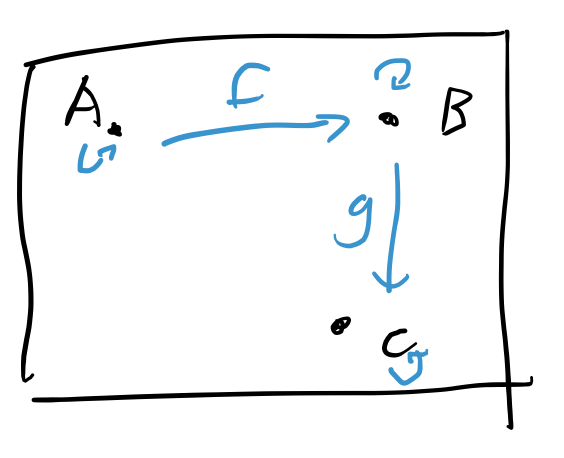
\includegraphics[width=0.4\linewidth]{fig/simple-cat1.png}
\end{center}
Morphisms can be combined via \emph{composition},
which pastes together morphisms that are incident to each other to form new ones.
Composing $g$ after $f$ is denoted $g \circ f$, or sometimes more tersely as \(gf\).
The ordering is a bit confusing; I like to read $\circ$ as ``after''.
Pictorially, we can paste together edges $f$ and $g$ to get an edge $h$:
\begin{center}
  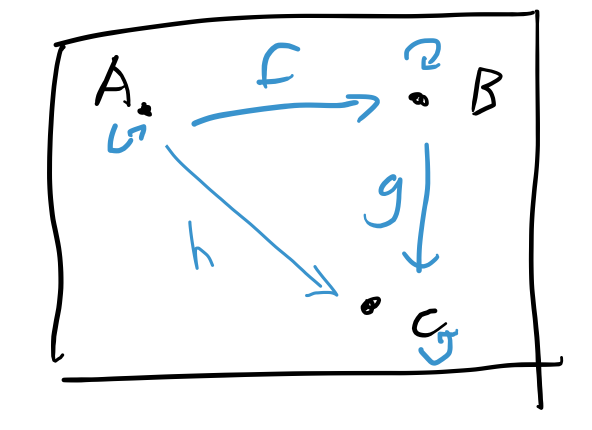
\includegraphics[width=0.4\linewidth]{fig/simple-cat2.png}
\end{center}
Categories satisfy several requirements that force them to behave nicely:
\begin{itemize}
  \item Every object has a self-loop called the \textbf{identity morphism},
  for an object $A$, we will denote its identity morphism as $\sf{id}_A$.
  This morphism must behave like an identity: for any morphism $A \xrightarrow{f} B$,
  it must be the case that $\sf{id}_B \circ f = f = f \circ \sf{id}_A$.
  \item Composition is \textbf{associative}, meaning that for any three morphisms
  $A \xrightarrow{f} B$, $B \xrightarrow{g} C$, $C \xrightarrow{h} D$,
  it is the case that $(f \circ g) \circ h = f \circ (g \circ h)$.
\end{itemize}
Summing up,\footnote{This definition of a category is one of many possible definitions. 
You may have seen different ones. This definition is used by \citep{crole1993categories}; 
different ones are used by \citep{mac1998categories}.}
\begin{definition}[Category]
  \sloppy
  A category is a tuple \((O,M,\mathsf{dom},\mathsf{cod},\mathsf{id},\mathsf{comp})\)
  where
  \begin{itemize}[noitemsep]
  \item $O$ is a set whose elements are called ``objects''
  \item $M$ is a set whose elements are called ``morphisms''
  \item $\mathsf{dom} : M\to O$
  \item $\mathsf{cod} : M \to O$
  \item $\mathsf{id} : O\to M$
  \item $\mathsf{comp} : \{(f,g) \in M \times M \mid \mathsf{dom}(f) = \mathsf{cod}(g)\} \to M$
  \end{itemize}
  such that
  \begin{itemize}[noitemsep]
  \item For all \(f\) and \(g\) in \(M\) such that \(\mathsf{dom}(f) = \mathsf{cod}(g)\)
    it holds that
    \[
    \mathsf{dom}(\mathsf{comp}(f,g)) = \mathsf{dom}(g)
    \quad\text{and}\quad
    \mathsf{cod}(\mathsf{comp}(f,g)) = \mathsf{cod}(f)
    \]
  \item For all \(X\) in \(O\) it holds that \(\mathsf{dom}(\mathsf{id}_X) = \mathsf{cod}(\mathsf{id}_X) = X\)
  \item For all $f,g,h$ in $M$ such that
  $\mathsf{dom}(f) = \mathsf{cod}(g)$ and\\
  $\mathsf{dom}(g) = \mathsf{cod}(h)$, it holds that
  $$\mathsf{comp}(f,\mathsf{comp}(g,h)) = \mathsf{comp}(\mathsf{comp}(f,g),h)$$
  \item For all $f$ in $M$ it holds that $$\mathsf{comp}(f,\mathsf{id}_{\mathsf{dom}(f)})=f=\mathsf{comp}(\mathsf{id}_{\mathsf{cod}(f)}, f)$$
  \end{itemize}
\end{definition}

\section{Our first metalanguage}

With a precise definition of category in hand, we are now ready to meet our first
``metalanguage''.

\marginnote{Set theorists may raise an eyebrow at
      the phrase ``set of finite sets'' in this definition.
      Strictly speaking, the set of finite sets does not form a set.
      But it is not that big of a deal:
      many workarounds are available.
      For instance, one could consider just finite subsets of \(\N\),
      or the set of \emph{hereditarily finite sets}
      (defined to be the union \(\bigcup_{n\in\N} \wp^n(\varnothing)\)).
      }
\begin{definition}[the category \(\FinSet\) of finite sets]
  \sloppy
  Let \(\FinSet\) be the category \((O,M,\dom,\cod,\circ,\idt)\)
  where \begin{itemize}[noitemsep]
  \item \(O\) is the set of finite
    sets.
  \item \(M\) is the set of tuples \((A,f,B)\) where \(A\) and \(B\)
    are finite sets
    and \(f\) is a function from \(A\) to \(B\).
  \item \(\dom\) is the function \(\dom(A,f,B) = A\).
  \item \(\cod\) is the function \(\dom(A,f,B) = B\).
  \item \(\circ\) is the function \((B,f,C)\circ(A,g,B) = (A,f\circ g,C)\)
    where \(f\circ g\) is the ordinary function composition of \(f\) and \(g\),
    well defined because the domain of \(f\) matches the codomain of \(g\).
  \item \(\idt_A\) is \((A,i,A)\) where \(i\) is the identity function on \(A\).
  \end{itemize}
\end{definition}

The category laws are satisfied because function composition is associative
  and composing a function with the identity function does nothing.

Mathematically, \(\FinSet\) provides a categorical home for finite set theory.
As a metalanguage, \(\FinSet\) embodies \emph{finite purely functional programming}.
For instance,
the following is a picture of the negation function \(f : \{T,F\} \to \{T,F\}\) 
in the category \(\FinSet\):

\begin{center}
  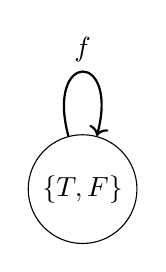
\begin{tikzpicture}
    % Define the node
    \node[circle, draw] (A) at (0,0) {$\{T,F\}$};
    
    % Draw self loop
    \draw[->, thick] (A) to[loop above] node[above] {$f$} (A);

\end{tikzpicture}
\end{center}

The above picture tells is that there \emph{is} a morphism called $f$, 
but it does not tell us anything about the \emph{content} of $f$. In particular, 
it is useful to know how $f$ maps elements of its domain to its codomain. 
To see this, we can draw the \textbf{internal picture} of this category
that visualizes the computational content of its morphisms:\footnote{Not 
all categories will have nice internal pictures, and different kinds of category 
will have their own visual language for describing their morphisms.}

\begin{center}
 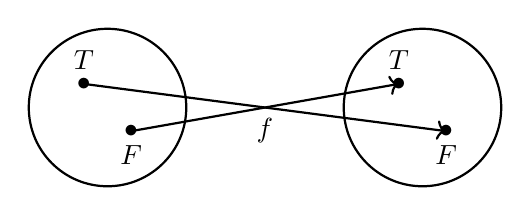
\begin{tikzpicture}
  % First circle with T and F dots
  \draw[thick] (0,0) circle (1);
  \node at (-0.3,0.3) {$\bullet$};
  \node at (-0.3,0.6) {$T$};
  \node at (0.3,-0.3) {$\bullet$};
  \node at (0.3,-0.6) {$F$};
  
  % Second circle with T and F dots
  \draw[thick] (4,0) circle (1);
  \node (T2) at (3.7,0.3) {$\bullet$};
  \node at (3.7,0.6) {$T$};
  \node (F2) at (4.3,-0.3) {$\bullet$};
  \node at (4.3,-0.6) {$F$};
  
    % Arrow from T on the left to F on the right
    \draw[->, thick] (-0.3,0.3) -- (4.3,-0.3);
    
    % Arrow from F on the left to T on the right
    \draw[->, thick] (0.3,-0.3) -- (3.7,0.3) node[midway, below] {$f$};
\end{tikzpicture}
\end{center}

Do not confuse the internal picture of a category with its picture: the internal 
picture ``peers inside objects'', and will not generalize to all kinds of categories.
This internal picture visualizes how the map $f$ behaves. A crucial 
piece information that this internal picture conveys is when two morphisms 
in \(\FinSet\) are equal: it is when they are \emph{extensionally equal}.

\todo: internal picture of \(\mathsf{not} \circ \mathsf{not} = \mathsf{id}\)


\section{Gaining intuition for categories}

The definition of category is highly abstract---and necessarily so, in order to be general enough
to accommodate all of the metalanguages just mentioned.
Next time, we will see how this level of abstraction allows for
clean axiomatizations of the various kinds of ``features'' that a metalanguage may support,
in the form of so-called ``universal constructions.''
This is what gives category theory its unifying power.

As preparation, we will first need to become quite comfortable working
with categories in the abstract. To do this, it is key to
have in mind a few representative examples of categories
to draw intuition from.

\subsection{Categories as graphs}

The first perspective on categories, which is perhaps most
comfortable to computer scientists, is that they are ``directed multigraphs with extra structure.''
Objects are vertices and morphisms are edges.
On top of this basic graph structure, categories come with a
composition operation that pastes two incident edges together to form a third,
and identity morphisms \(\mathsf{id}_A\) that form self-loops centered at each vertex \(A\).
The category laws then say that pasting of edges is an associative operation,
and that pasting with an identity morphism does nothing.
This provides nice visual intuition, and a large stock of example categories.
In fact,
\begin{construction}
  Every directed multigraph can be turned into a category.
\end{construction}
\begin{proof}
  Let \(G\) be a directed multigraph,
  encoded as a tuple \((V,E,\mathsf{src},\mathsf{trg})\)
  where \(V\) is the set of vertices, \(E\) is the set of edges,
  and \(\mathsf{src},\mathsf{trg}\) are functions \(E\to V\)
  that send each edge to its source and target vertices respectively.
  The graph \(G\) can be used to define a category
  \[
  \mathsf{paths}(G) = (O,M,\dom,\cod,\circ,\idt)
  \]
  where
  \begin{itemize}
  \item \(O = V\)
  \item \(M\) is the set of paths in \(G\),
    which are tuples \((v_s,[e_1,\dots,e_n],v_t)\)
    where \(v_s,v_t\) are vertices and \(e_1,\dots,e_n\) is a list of edges satisfying
    \(\mathsf{src}(e_1) = v_s\) and \(\mathsf{trg}(e_n) = v_t\)
    and \(\mathsf{trg}(e_i) = \mathsf{src}(e_{i+1})\)
    for all \(1\le i < n\).
  \item \(\dom : M \to O\) is the function \(\dom(v_s,[e_1,\dots,e_n],v_t) = v_s\)
  \item \(\cod : M \to O\) is the function \(\cod(v_s,[e_1,\dots,e_n],v_t) = v_t\)
  \item \(\circ\) concatenates paths:
    \((v_t,[f_1,\dots,f_n],v_u)\circ(v_s,[e_1,\dots,e_m],v_t) = (v_s,[e_1,\dots,e_m,f_1,\dots,f_n],v_u)\).
    Note that this is well-defined because the two paths \(\vec f\) and \(\vec e\) line up tip-to-tail.
    Note also that \(\vec e\) comes before \(\vec f\) in the concatenated path, due to the reversal of order
    of arguments to \(\circ\).
  \item \(\idt_v\) is the empty path \((v,[],v)\) starting and ending at \(v\).
  \end{itemize}
  The category laws are satisfied because concatenation of paths is associative and concatenating a path with the
  empty path does nothing.
\end{proof}
\begin{note}
  It is essential that morphisms are \emph{paths} in this construction, and not edges!
  Otherwise, it would be unclear how to define composition and identity.
\end{note}

\subsection{A Difference Between Categories and Directed Multigraphs}

A key difference between categories and graphs is that
two morphisms in a category that come from
different ``paths'' may nonetheless be equal.
For example, the following two ``paths'' through \(\FinSet\)
are actually the same, because negating a Boolean twice is the same as doing nothing:
\[% https://tikzcd.yichuanshen.de/#N4Igdg9gJgpgziAXAbVABwnAlgFyxMJZABgBpiBdUkANwEMAbAVxiRAB13gAVUgMU4BfEINLpMufIRQAmclVqMWbTj35CRYkBmx4CRAIykDC+s1aIOXXgPbDBCmFADm8IqABmAJwgBbJGQgOBBIRormKuy+dDgAFnAewJA49lrefqHUwUhy4cqWnNFxCUkQKZqePv6IgdmIuWb5VlhQOAD6wKo2QsLUDHQARjAMAAoSetIgXljOsTgiFIJAA
\begin{tikzcd}
{\{T,F\}} \arrow[rr, "\mathsf{not}"] \arrow[rd, "{\idt_{\{T,F\}}}"'] &           & {\{T,F\}} \arrow[ld, "\mathsf{not}"] \\
                                                                     & {\{T,F\}} &
\end{tikzcd}\]
This relationship between the paths \(\mathsf{not}\circ \mathsf{not}\) and \(\idt_{\{T,F\}}\)
is often conveyed by saying that the triangle above is ``filled in'', or ``commutes''.
The intuition being that one can then ``continuously deform''
\(\mathsf{not}\circ\mathsf{not}\) into \(\idt_{\{T,F\}}\),
by ``dragging'' it through the filled in triangle.

This idea is a handy visual tool for organizing categorical information
and for conducting proofs.

\subsection{Categories as orders}

A special case of a multigraph is a graph, where there is \emph{at most one} arrow between any given pair of vertices.
This leads us to the second class of important examples of a category:
\begin{definition}[preorder]
  \sloppy
  A preorder is a pair \((X,\preceq)\)
  where \(X\) is a set and \(\preceq\)
  is a binary relation on \(X\)
  that is reflexive (\(x\preceq x\) for all \(x\) in \(X\))
  and transitive (if \(x \preceq y\) and \(y\preceq z\) then \(x \preceq z\)).
\end{definition}
Preorders are often fruitfully drawn as \emph{Hasse diagrams}.
%% An object is like an element of a preorder
%% and a morphism \(x\to y\) is like a ``proof'' that \(x\le y\).
A simple example is the set \(\N\) of natural numbers,
ordered by \(m\preceq n\) if \(m\) is less than or equal to \(n\).
We can draw this preorder as follows:
\[
% https://tikzcd.yichuanshen.de/#N4Igdg9gJgpgziAXAbVABwnAlgFyxMJZABgBoBmAXVJADcBDAGwFcYkRiQBfU9TXfIRRkATNTpNW7AIzdeIDNjwEiZaeIYs2iECLl8lg1aWIbJ2kAB1LtKBBwIu4mFADm8IqABmAJwgBbJHIaHAgkERoACxh6KHZIMDYebz9AxAiQUKRpKJi4nQSk+V8A7JCwxDIQaNj4giTKLiA
\begin{tikzcd}
\vdots \arrow[d, no head] \\
2 \arrow[d, no head]      \\
1 \arrow[d, no head]      \\
0
\end{tikzcd}\]
Hasse diagrams are read bottom-up, with the least elements 
on the bottom and the greatest elements on the top. 
An undirected edge is drawn between elements with no elements 
between them (this is why we have no edge from 0 to 2 in the above figure).
A more visually interesting preorder on \(\N\)
is to define \(m \preceq n\) if \(m\) is a \emph{divisor} of \(n\).
This preorder looks less like a straight line and more like a lattice:
\[
% https://tikzcd.yichuanshen.de/#N4Igdg9gJgpgziAXAbVABwnAlgFyxMJZARgBoBmAXVJADcBDAGwFcYkRiQBfU9TXfIRQAGUgCZqdJq3ZjuvEBmx4CRMhJoMWbRCHLy+ywUTHjJWmboCsBxfxVDko4uek6QANltKBqlGRdNN3ZiYW97YxRTQKltEJseQ19HUWFXON0AHUzaKAgcBES7Iz9kUzSgjJBs3PzChR8HNVIK2MtqnLyC7kkYKABzeCJQADMAJwgAWyQyEBwIJFEQAAsYeih2SDA2IvGppFM5hcQl1fXNgh2FPenEchp5xZozjd0tq9GJ248H48OXi7bWw3JA-I5Ie4rNavcCXYFfJBWX4zZ7QwEfEAgxBI8F3VHnN5w3YIxAAFmRiH+aMJQOJ+zJFNmAJpGKx5NxAHZ8TD3vD6WDHogABzc9F8244wUATlFLJ6XCAA
\begin{tikzcd}
\vdots                                                      & \vdots                                                        & \vdots                                                       \\
6 \arrow[rd, no head] \arrow[d, no head] \arrow[u, no head] & 10 \arrow[ld, no head] \arrow[rd, no head] \arrow[u, no head] & 15 \arrow[ld, no head] \arrow[d, no head] \arrow[u, no head] \\
2 \arrow[rd, no head]                                       & 3 \arrow[d, no head]                                          & 5 \arrow[ld, no head]                                        \\
                                                            & 1                                                             &
\end{tikzcd}
\]
Preorders don't have to be discrete either: the real numbers \(\R\),
for instance, form a preorder with \(x \preceq y\) if \(x\) is less than or equal to \(y\). This is a little harder to draw.

A preorder that arises frequently in PL is the preorder of
\emph{run-time environments}.
It is common to model these environments
as partial functions \(\rho : \mathsf{Var} \rightharpoonup \mathsf{Val}\),
assigning to each program variable \(x \in \mathsf{Var}\)
a concrete value \(\rho(x)\).
These substitutions form a preorder, with \(\rho \preceq \rho'\)
if \(\rho\) is a subset of \(\rho'\), in the sense that all the 
variables in $\rho$ are in $\rho'$ and mapped to the same values.
%% \item Heaps under disjoint union: let \(\mathsf{Heap}\) be the category
%%   whose objects are substitutions \(\gamma\),
%%   i.e., partial functions \(\mathsf{Loc} \rightharpoonup \Z\),
%%   and whose morphisms from \(h\) to \(h'\)
%%   are heaps \(h_{\mathsf{diff}}\) such that \(h \uplus h_{\mathsf{diff}} = h\).

Preorders forms a category:
\begin{construction} \label{prop:every-preorder-is-a-category}
  Every preorder can be turned into a category.
  \label{eq:const-preorder}
\end{construction}
\begin{proof}
  For any preorder \((X,\preceq)\), there is a category
  \[
    \mathsf{order}(X,\preceq) = (O,M,\dom,\cod,\circ,\idt)
  \]
  where
  \begin{itemize}
    \item \(O = X\).
    \item \(M = (\preceq)\) (recall that a binary relation like \(\preceq\)
      can be thought of as a set of pairs, with \((x,y) \in (\preceq)\)
      if and only if \(x\preceq y\)).
    \item \(\dom\) is the function \(\dom(x,y) = x\).
    \item \(\cod\) is the function \(\cod(x,y) = y\).
    \item \(\circ\) is the function defined by \((y,z)\circ(x,y) = (x,z)\).
      Note that we may assume that the two arguments to \(\circ\)
      share a component \(y\) in this definition because of the assumption
      that \((y,z)\) and \((x,y)\) are composable.
      Note also that the composite \((x,z)\) is indeed well-defined
      this is well defined by the transitivity of \(\preceq\).
    \item \(\idt_x\) is the pair \((x,x)\), which forms a valid morphpism
      by reflexivity of \(\preceq\).
  \end{itemize}
  The category laws are satisfied automatically,
  as there can only be at most one morphism between any two objects.\footnote{Pause: 
  why is this the case?}
\end{proof}
\noindent
The intuitive import of Proposition~\ref{prop:every-preorder-is-a-category}
is that every category can be thought of as a kind of preorder,\footnote{\emph{Reminder}: not all 
categories directly correspond to some preorder construction, since there can be multiple 
morphisms between objects in a general category. A category with at most 1 morphism between 
any 2 objects is called a \emph{thin category}, and it does correspond to some preorder.}
where the existence of a morphism \(A\xrightarrow{f} B\)
expresses that \(A\) is in some sense ``less than or equal to'' \(B\).
Thinking of categories in this way leads to interesting questions like:
\begin{itemize}
\item
  Does a category have a ``smallest'' or ``largest'' object?
  For instance, the smallest runtime environment is the empty environment $\emptyset$
  with no variables in it.
\item Does a category have ``ascending sequences''?
  For example, 
  \begin{align}
   \emptyset \subseteq \{x\mapsto A\} \subseteq \{x\mapsto A, y\mapsto B\} \subseteq \dots 
   \label{eq:env-seq}
  \end{align}
  is an ascending sequence in the preorder of runtime environments.
\item  Does a category have ``limit'' objects, like suprema or infima?  For
  instance, you probably know from calculus that there limits in \(\R\): for
  example, the sequence $\frac{1}{2}, \frac{1}{4}, \frac{1}{8},
  \frac{1}{16}\cdots$ approaches 0 in the limit.  A very interesting question is:
  which categories ``have limits'', in the sense that such sequences always
  converge to some object in the category?

  An example of a situation where there is no limit is the sequence in
  \cref{eq:env-seq}.  The set of environments grows and grows, and since there
  is no notion of a ``greatest environment'', there is no limit to this
  sequence.
\item
  Given two categories, is there a notion of ``monotone map'' between them?
\end{itemize}

Each of the above observations is foreshadowing a notion of a ``universal construction''
in a category, which we will explore in the following lectures.

\subsection{Categories as algebras}

Whereas preorders are like multigraphs where there is at most one \emph{edge}
between any two vertices,
the opposite extreme is a multigraph with exactly one \emph{vertex},
so that all edges are self-loops:
% https://q.uiver.app/#q=WzAsMSxbMCwwLCJcXGJ1bGxldCJdLFswLDBdLFswLDAsIiIsMCx7InJhZGl1cyI6MX1dLFswLDAsIiIsMCx7InJhZGl1cyI6NX1dXQ==
\begin{equation}
\begin{aligned}
\begin{tikzcd}
	\star
	\arrow[from=1-1, to=1-1, loop, in=55, out=125, distance=10mm]
	\arrow[from=1-1, to=1-1, loop, in=60, out=120, distance=5mm]
	\arrow[from=1-1, to=1-1, loop, in=50, out=130, distance=15mm]
\end{tikzcd}
\end{aligned}
\end{equation}
Categories of this shape form our final class of important example:
a special kind of algebraic structure called a \emph{monoid}.
\begin{definition}[monoid]
  A monoid is a tuple \((X,\bullet,e)\)
  where \(\bullet\) is a binary operation on \(X\)
  (a function \(X \times X \to X\))
  that is associative (\(x\bullet (y\bullet z) = (x\bullet y) \bullet z\))
  and has \(e\) as a unit (\(x\bullet e = x\) and \(e\bullet x = x\)).
\end{definition}
A simple example of a monoid is \((\N,+,0)\),
the monoid of natural numbers under addition.
This forms a monoid because addition of natural numbers is associative
and has zero as a unit.

An example that is closer to PL
comes from the semantics of imperative programs.
It is common to interpret an imperative program
as a function \(S \to S\), where \(S\) is a set of
memory states.
For example, the program
\[
  x := x + 1;
\]
can be interpreted
as a function that sends a memory state \(s\)
to a new memory state \(s'\) in which
the value of \(x\) has been incremented by \(1\).
The functions \(S \to S\) form a monoid
\((S\to S,\bullet,\mathsf{id})\),
where the monoid operation is given by \(f \bullet g = g \circ f\)
(note the reversal!),
corresponding to the sequencing of the programs \(f\) and \(g\),
and the identity element is the identity function on \(S\),
corresponding to the empty program that does nothing.

Algebraic identities capture program rewrites for this imperative language.
For example, if \(f\) is the interpretation of \(x := 0\)
and \(g\) is the interpretation of \(y := 1\),
and \(x\) and \(y\) are distinct program variables,
then the program equation
\begin{equation}
  \left(\begin{aligned}
    &x := 0 \\
    &y := 1
  \end{aligned}\right)
  \equiv
  \left(\begin{aligned}
    &y := 1 \\
    &x := 0
  \end{aligned}\right)
\end{equation}
can be expressed as the algebraic identity \(g \circ f = f \circ g\).

\begin{construction} \label{prop:every-monoid-is-a-category}
  Every monoid can be turned into a category.
\end{construction}
\begin{proof}
  For any monoid \((X,\bullet,e)\) there is a category
  \[
    \mathsf{mon}(X,\bullet,e) = (O,M,\dom,\cod,\circ,\idt)
  \]
  where
  \begin{itemize}
  \item \(O = \{\star\}\), a singleton set with a single dedicated element \(\star\).
    \marginnote{Technically set theory does not contain stars in it.
    But this is no matter.
    The symbol \(\star\) can be interpreted as any object of
    your choice---all that matters
    is that \(O\) is a singleton set.
    For instance, one could set \(\star =
    \varnothing\).
    }
  \item \(M = X\)
  \item \(\dom(M) = \star\)
  \item \(\cod(M) = \star\)
  \item Composition is defined by \(x \circ y = x \bullet y\)
  \item \(\idt_\star = e\)
  \end{itemize}
  The category laws follow from the associativity of \((\bullet)\)
  and that it has \(e\) as a unit.
\end{proof}
\begin{note}
  It is very important that the set of objects \(O\) is a singleton set \(\{\star\}\).
  A natural thought one might have is that the set of objects should be the set \(X\) of elements of the monoid.
  But this in fact does not work: what would be the morphisms?

  There is actually a good reason why the set of objects is the seemingly-arbitrary singleton set \(\{\star\}\) in this construction.
  It comes from the fact that a monoid is what is called a \emph{single-sorted} algebraic structure; hence \(\{\star\}\)
  is a set with a single element.
\end{note}
The intuitive import of
Proposition~\ref{prop:every-monoid-is-a-category} is that
every category can be thought of as a kind of algebraic structure,
where composition is like ``multiplication''
and identity morphisms are like ``multiplicative units''.

The algebraic perspective leads to questions like:
given an equation between morphisms containing some unknowns,
are there zero, one, or infinitely many solutions?
When can I ``cancel'' a morphism from both sides of an equation (e.g., from \(fg = fh\) deduce \(g=h\),
or from \(fh = gh\) deduce \(f=g\))?
When does a morphism have an ``inverse''?
When can a morphism \(f\) be ``factored'' into two pieces, \(f = gh\)?

\section{Putting intuitions to the test}

We conclude this section by illustrating each of the three perspectives
on categories on the following
\textbf{categorification}\footnote{The idea of ``categorification'' is to 
cast a notion one is familiar with -- like ``subset inclusion'' into 
the language of objects and morphisms. This is a very important idea 
in category theory because it allows one to take familiar concepts 
and apply them to unfamiliar categories.} of
a basic concept from set theory: subset inclusion.
\begin{proposition} \label{prop:subset-leq-iff-triangle}
Suppose \(U\) and \(V\) are subsets of a finite set \(X\).
Then \(U \subseteq V\) if and only if
there exists a dashed \(\FinSet\)-morphism \(f\)
such that \(f \circ v = u\),
where \(u\) and \(v\) are the \(\FinSet\)-morphisms
corresponding to the inclusion functions\footnote{A function $f : X \to Y$ 
is an \emph{inclusion function} (also called an ``injective map'') if 
each element of $X$ is mapped to a unique element in $Y$. 
All inclusion functions have a ``left inverse'': 
there exists a function $g$ such that $g \circ f = \mathsf{id}_X$.
Inclusion maps are rendered using tailed arrows.} \(U \to X\) and \(V \to X\)
respectively:
\begin{equation}
  % https://tikzcd.yichuanshen.de/#N4Igdg9gJgpgziAXAbVABwnAlgFyxMJZABgBpiBdUkANwEMAbAVxiRAFUQBfU9TXfIRQAmclVqMWbAGrdeIDNjwEiARlKrx9Zq0QgAGt3EwoAc3hFQAMwBOEALZIyIHBCSiXdLAzY4vP6m0pPSYQagY6ACMYBgAFfmUhEBssUwALHDlrO0dEdRc3RA8-b19-MIkdNhoskFsHJ2pXJHySnz1IMFZwrC62KDo4NJMKoN06oy4gA
\begin{tikzcd}
U \arrow[rd, "u"', tail] \arrow[rr, "f", dashed] &   & V \arrow[ld, "v", tail] \\
                                                 & X &
\end{tikzcd}
\end{equation}
\end{proposition}
You will prove Proposition~\ref{prop:subset-leq-iff-triangle} in the homework.
As preparation,
let's appreciate what it is saying: a basic set theoretic
property \(U\subseteq V\) about finite subsets
can be recast in terms of a purely category-theoretic property
about \(\FinSet\).
This categorification takes roughly two steps.
The first step is to express the subsets \(U\) and \(V\)
as morphisms \(u\) and \(v\).
The second step is to express \(U\subseteq V\)
as a property of the morphisms \(u\) and \(v\).
Let's try to get some intuition for what this property is saying
from each of the perspectives we've developed so far.
\begin{itemize}
\item Graphically, it says that the morphisms \(u\) and \(v\)
  fit into a triangle with \(f\) that is ``filled in''.
\item Order-theoretically, it says that the morphism \(u\) is somehow
  ``less than or equal to'' \(v\), by virtue of there being a dashed morphism
  \(f\) witnessing this order relationship.

  We can make this formal as follows.
  For any finite set \(X\), one can construct a category \(\mathsf{Sub}(X)\).
  The objects of this category are tuples \((U,u)\) where \(U\) is a subset of \(X\)
  and \(u\) is the function \(U \to X\) defined by \(u(x) = x\);
  i.e., \(u\) is the canonical inclusion function of \(U\) into \(X\).
  The morphisms of this category are, roughly speaking,
  pictures of the following shape:
  \[
  % https://tikzcd.yichuanshen.de/#N4Igdg9gJgpgziAXAbVABwnAlgFyxMJZABgBpiBdUkANwEMAbAVxiRAFUQBfU9TXfIRQBGUsKq1GLNgA1uvEBmx4CRAEzkJ9Zq0QgAatwkwoAc3hFQAMwBOEALZIyIHBCSjJOtkxDUGdACMYBgAFfhUhEBssUwALHHlrO0dEDRc3RA9taT0aRJBbBydqVyQ07N0Coy4gA
\begin{tikzcd}
U \arrow[rd, "u"'] \arrow[rr, "f"] &   & V \arrow[ld, "v"] \\
                                   & X &
\end{tikzcd}
  \]
  Formally, a morphism is a tuple \((U,u,f,V,v)\)
  where \(U\) and \(V\) are subsets of \(X\),
  \(u : U \to X\) and \(v : V \to X\) are the canonical inclusions,
  and \(f\) is a function \(U \to V\)
  such that \(v \circ f = u\).
  Each morphism \((U,u,f,V,v)\) has domain \((U,u)\)
  and codomain \((V,v)\).

  Now Proposition~\ref{prop:subset-leq-iff-triangle}
  says that \(U\subseteq V\) if and only if there is a morphism from \((U,u)\)
  to \((V,v)\) in the category \(\mathsf{Sub}(X)\),
  witnessing the fact that \((U,u)\) is ``less than or equal to'' \((V,v)\).

\item Algebraically, it says that the equation \(u = f \circ v\)
  has a solution in the unknown \(f\).
\end{itemize}
Let's see each of these in action on the following proof.
\begin{proposition}
  If \(U\subseteq V\) and \(V \subseteq W\) then \(U\subseteq W\).
\end{proposition}
Each perspective lends itself to a different proof strategy.
\begin{itemize}
\item Graphically, you paste two filled in triangles to get a bigger filled in triangle.
\item Order-theoretically, you use the fact that \(\mathsf{Sub}(X)\), as a category,
  has composition.
\item Algebraically, you use that \(u = vf = wvg\) provides a solution to \(u = wh\).
\end{itemize}

%% \item Refinement corresponds to solvability of an equation that looks like a square.
%%   Suppose you have a subset \(U\) of a finite set \(X\),
%%   a subset \(V\) of a finite set \(Y\),
%%   and a function \(f : X \to Y\).
%%   Let \(u : U \rightarrowtail X\) and \(v : V \rightarrowtail Y\) be the relevant inclusions.

%%   Suppose \(f\) satisfies the property that,
%%   for all \(x \in U\), it holds that \(f(x) \in V\).
%%   This can be expressed as saying that the equation
%%   \(fu = vg\) is \emph{solvable} in the unknown \(g\).
%%   Diagramatically:
%%   \[
%%   % https://tikzcd.yichuanshen.de/#N4Igdg9gJgpgziAXAbVABwnAlgFyxMJZABgBpiBdUkANwEMAbAVxiRAFUQBfU9TXfIRQBGclVqMWbAGrdeIDNjwEiZYePrNWiEAA05fJYKKj11TVJ0BNbuJhQA5vCKgAZgCcIAWyRkQOCCQAJmocOiwGNjCIkHNJbRAmWJAGOgAjGAYABX5lIRB3LAcACxwDEA9vJFF-QMQAZlDwyJ1oyLitNhpyyp9EPwDqjssQBx7PPpDapEaJTp1XZNSM7NzjHUKSsq4KLiA
%% \begin{tikzcd}
%% U \arrow[d, "u"', tail] \arrow[r, "g"] & V \arrow[d, "v", tail] \\
%% X \arrow[r, "f"']                      & Y
%% \end{tikzcd}
%%   \]
%%   This situation actually comes up quite a lot in PL,
%%   as we will see when we discuss logical relations.

%%   (By the way, the solution \(g\), if it exists, must be the \emph{only} solution to this equation,
%%   as if one finds \(g\) and \(g'\) such that \(fu = vg\) and \(fu = vg'\), then \(vg=fu=vg'\),
%%   and left-cancellativity of \(v\) implies \(g = g'\).)

\subsection{Some fun exercises}

\begin{itemize}
\item Explicitly write down the monoid \((\N,+,0)\) as a category.
\item Solve the equation \(c \circ (x := x + 1) = (x := x + 2)\) for \(c\).
  Can you find any other solutions?
\item Try to come up with an English description of what it means for an Imp command to be ``left'' or ``right'' cancellable
\item Prove Proposition~\ref{prop:subset-leq-iff-triangle}.
\item Show that the functions \(u,v\) in Proposition~\ref{prop:subset-leq-iff-triangle}
  are left-cancellable as morphisms of \(\FinSet\).
\end{itemize}

\chapter{Universal Constructions I}
We've been hinting at the utility of knowing that categories that have certain
special objects in them. For example, if we want to give a category that lets us
validate equations of programming languages, that category will need to be able 
to represent the many features that programs might have: products, sums, 
functions, etc. Here we will introduce the essential idea of a \textbf{universal 
construction} that characterizes when categories contain these special objects.

\section{Terminal objects \& the unit type}
Recall that when designing categorical semantics for programming languages we
associate types and typing contexts with objects in the category and terms with
morphisms. Concretely, if we have a well-typed term $\Gamma \vdash e : A$,
its interpretation $\dbracket{\Gamma \vdash e : A}$ is a morphism
$\dbracket{\Gamma} \xrightarrow{\dbracket{e}} \dbracket{A}$.
Previously, we showed how \(\FinSet\) can be used to give an interpretation 
to \ref{lang:calc} programs by associating types like the unit type $\plUnit$
with special sets, like a set containing only a single element $\{\star\}$.
But, what if we want to see if categories other than $\FinSet$ can give give a 
reasonable interpretation for $\plUnit$?

To proceed, let's pick a particular object $\dbracket{\plUnit}$ 
in a category $\calC$ and explore what properties it needs to have in order 
to be ``$\plUnit$-like'':
\begin{itemize}
  \item \textbf{Fact 1, Introduction rules}: It must be possible in any typing context to
  produce a value of type $\plUnit$.  This tells us that for any context
  $\Gamma$, there must exist a $\calC$-morphism
  $\dbracket{\Gamma} \to \dbracket{\plUnit}$.
  For example, it must 
  be the case that 
  $\dbracket{\Gamma} \xrightarrow{\dbracket{\plunit}} \dbracket{\plUnit}$.

  \item \textbf{Fact 2, Equational laws}: Since \ref{lang:calc} has no effects, 
  it is the case that if $\Gamma \vdash e : \plUnit$, then it is indistinguishable 
  from the term $\plunit$. This is called \textbf{eta equality}, and we write
  this as $e \equiv \plunit$.\footnote{The symbol ``$\equiv$'' means ``is
  equationally equal to''.} Eta equality is an equational law that characterizes
  how a $\plUnit$ term must behave. Now for an insight: \emph{these equational
  laws are translated into morphism equalities}. It must be that, for any
  morphism $\dbracket{\Gamma} \xrightarrow{\dbracket{e}} \dbracket{\plUnit}$, it
  is the case that $\dbracket{e} = \dbracket{\plunit}$.  In other words, the
  morphism $\dbracket{\Gamma} \xrightarrow{\dbracket{\plunit}} \plUnit$ must be
  unique.
\end{itemize}

These two properties can be packaged up into a nice concise definition:

\begin{definition}[Terminal object] 
  Let $T$ be an object in a category $\calC$. 
  An object $T$ in $\calC$ is called a terminal object
  if, for every other object $A$ in $\calC$ there exists a unique 
  morphism $A \xrightarrow{\langle \rangle} T$. Graphically,

  \begin{center}
% https://tikzcd.yichuanshen.de/#N4Igdg9gJgpgziAXAbVABwnAlgFyxMJZABgBpiBdUkANwEMAbAVxiRAEEQBfU9TXfIRQBGclVqMWbACrdxMKAHN4RUADMAThAC2SMiBwQkokAyxhWiEHAhmoIagzoAjGAwAK-PATYMYanAcJZksQAB0wmAAPLDgcOABCOS4gA
\begin{tikzcd}
  A \arrow[r, "\exists!"] & T
  \end{tikzcd}
\end{center}
\end{definition}

Let's pause to remark on the three categorical interpretations 
of terminal objects $T$:
\begin{itemize}
  \item Graphically, an object is terminal if (1) there is an arrow from 
  every other object to it, and (2) it ``thins all parallel
  arrows'', meaning that if we have a situation like the following for 
  and morphisms $X \xrightarrow{f} T, X \xrightarrow{g} T$:
  \begin{align*}
    % https://tikzcd.yichuanshen.de/#N4Igdg9gJgpgziAXAbVABwnAlgFyxMJZABgBpiBdUkANwEMAbAVxiRABUQBfU9TXfIRRkAjFVqMWbABrdxMKAHN4RUADMAThAC2SEdRwQkZEACMYYKEgC0AZhMM65hgAV+eAmw1ZFACxwg1PTMrIggity8IJo6egZGiCbmlkj21I7ObtgeQiAMMGoBQZKh0XJcQA
\begin{tikzcd}
  T                                                       \\
  X \arrow[u, "g"', bend right] \arrow[u, "f", bend left]
  \end{tikzcd},
  \end{align*}
  then we know that $f = g$.
  \item The order-theoretic perspective is that the terminal object 
  is the ``greatest object'' in the category.
  \item The algebraic perspective yields the natural equations:
  for any morphism from $A \xrightarrow{f} T$, it is the case 
  that $f = \langle \rangle$.
\end{itemize}

We say a category \textbf{has terminal objects} if there is an object in the
category that is a terminal object. This is our first example of a 
\textbf{universal construction}, which are special objects in categories 
characterized by their morphisms into them. We will see how universal 
constructions can be used to give interpretations to all the type 
formers we have seen so far. But, we can already see their utility: 
whether or not a particular category admits certain universal constructions
will immediately inform us of that category's suitability for modeling 
certain language properties.

\subsection{$\FinSet$ has terminal objects, isomorphisms}
We saw in previous lectures that we could use the singleton set 
$\{\star\}$ to give an interpretation to $\plUnit$ in $\FinSet$.
We can easily prove that $\{\star\}$ is a terminal object:
\begin{theorem}
  The singleton set $\{\star\}$ is terminal in $\FinSet$.
\end{theorem}
\begin{proof}
  \begin{itemize}
    \item Existence: The map $\_ \mapsto \{\star\}$ has the required type.
    \item Uniqueness: Suppose we have two morphisms $A \xrightarrow{f} \{\star\}$ and
    $A \xrightarrow{g} \{\star\}$. 
    Then by function extensionality we immediately have that $f = g$ 
    as set-functions, and so they are equal as $\FinSet$ morphisms.
  \end{itemize}
\end{proof}

Now you can observe the above proof and see that it immediately 
works for \emph{any} choice of singleton set: does this mean that $\FinSet$
has \emph{many terminal objects?} Yes, and no. \emph{Yes}, in the sense 
that there are indeed many valid choices of terminal object; but \emph{no}, 
in the sense that the choice itself does not (\emph{should} not!) actually 
matter. We capture this by the notion of isomorphism:

\begin{definition}[Isomorphism of objects]
  \sloppy
  Two objects $A$ and $B$ in a category $\calC$ are isomorphic if 
  there exist morphisms $A \xrightarrow{f} B$ and $B \xrightarrow{g} A$
  such that (1) $g \circ f = \id_A$ and (2) $f \circ g = \id_B$.
\end{definition}

We can immediately see that any two singleton sets in $\FinSet$ are isomorphic:
this proof is straightforward. What might be surprising is that this 
fact is true for all terminal objects:

\begin{theorem} \label{thm:terminal-object-unique}
  Terminal objects are unique up to isomorphism.
\end{theorem}
\begin{proof}
  Let $X$ and $Y$ be terminal objects in some category $\calC$. 
  Then there exists a pair of unique morphisms between them:

  \begin{center}
 % https://tikzcd.yichuanshen.de/#N4Igdg9gJgpgziAXAbVABwnAlgFyxMJZABgBpiBdUkANwEMAbAVxiRAA0QBfU9TXfIRQBGclVqMWbAJrdxMKAHN4RUADMAThAC2SMiBwQkokACMYYKEgDM++s1aIQAQjXdeITTuPVDe6uaWNnaSji6KclxAA
\begin{tikzcd}
  X \arrow[r, "!f", bend left] & Y \arrow[l, "!g", bend left]
  \end{tikzcd} 
\end{center}
By the fact that $X$ and $Y$ are terminal, they must also have unique identity
morphisms $\id_X$ and $\id_Y$. Then by the uniqueness of identity we have that $g \circ f = \id_X$ and $f \circ g = \id_Y$.
\end{proof}

This provides some evidence that the choice of terminal object does not matter.
  But are we done? Suppose we had two terminal objects \(T\) and \(T'\).
  By the above argument, we have that these two objects are isomorphic.
  But now another potential choice arises: what if there are multiple different
  \emph{isomorphisms} between \(T\) and \(T'\)?
  Then it could be that the choice to use \(T\) instead of \(T'\)
  may implicitly come with a choice of specific isomorphism as well.

  Luckily, terminal objects satisfy a stronger property
  which ensures that one's choice is terminal object is truly irrelevant.

\begin{proposition}
  Terminal objects are unique up to \emph{unique} isomorphism.
  That is, if \(T\) and \(T'\) are both terminal,
  then there is exactly one isomorphism
  \((f:T\to T',g:T'\to T)\)
  between \(T\) and \(T'\).
\end{proposition}
\begin{proof}
  Both \(f\) and \(g\), as constructed in the proof of
  \Cref{thm:terminal-object-unique},
  are the only possible morphisms \(T \to T'\) and \(T'\to T\)
  respectively. Thus they together form the only isomorphism
  between \(T\) and \(T'\).
\end{proof}

Later on, when we have the language for it, we will show that
all universal constructions are unique up to unique isomorphism
in this sense, and hence free of non-canonical choices.

% \subsection{Terminal objects for preorders}
% Universal constructions are one of the engines for analogy in category theory:
% very different-seeming concepts can be cast as instances of the same 
% universal construction, which can bring clarity to what each of those disparate 
% concepts means. When cast order-theoretically, the terminal object can 
% be thought of as ``the greatest object in a category.''
% % The first instance we will see of a universal construction is a \textbf{terminal 
% % object}, which can be thought of as ``the largest object in a category'' if one 
% % recalls the preorder intuition of morphisms. 

% An element of a preorder is the largest if it is greater than every other 
% element: i.e., there exists a morphism from every other element to it.
% This definition works for a general category: one could say an object is 
% largest if there exists a morphism from every other object into it.
% This characterization however doesn't take into account that there 
% can be more than 1 morphism between any two objects in a category: intuitively, 
% this means that one object can be greater than another in more than one way.

\section{Products}
Next we want to interpret product types $A \times B$. As before with the 
unit type, the typing rules for products forces the existence of certain morphisms,
and the equational theory of products forces equalities of certain morphisms.
The  introduction rule that describes how to create new products is:
\begin{mathpar}
\inferrule
    {\Gamma\vdash M : A
      \\
    \Gamma\vdash N : B
    }
    {\Gamma \vdash \plpair{M}{N} : A \pltimes B}~(\textsc{T-Pair})
\end{mathpar}
The elimination rules that break apart products are:
\begin{mathpar}
\inferrule
    {\Gamma\vdash M : A \pltimes B}
    {\Gamma \vdash \plfst{M} : A}~(\textsc{T-Fst})
\and
\inferrule
    {\Gamma\vdash M : A \pltimes B}
    {\Gamma \vdash \plsnd{M} : B}~(\textsc{T-Snd})
\end{mathpar}

These rules imply the existence of several morphisms that characterize 
what it means for for a special object $\dbracket{A \times B}$ to be a 
product. Reading off from the rules:
\begin{itemize}
  \item The \textsc{T-Pair} rules says that if there are 
  two morphisms $\dbracket{\Gamma} \mor{\dbracket{M}} \dbracket{A}$ and 
  $\dbracket{\Gamma} \mor{\dbracket{N}} \dbracket{B}$, 
  then there is a morphism $\dbracket{\Gamma} \mor{\dbracket{\langle M, N \rangle}} 
  \dbracket{A \times B}$.
  \item The \textsc{T-Fst} rule says that if there is a morphism 
  $\dbracket{\Gamma} \mor{\dbracket{M}} 
  \dbracket{A \times B}$, then there is a 
  morphism $\dbracket{\Gamma} \mor{\dbracket{\plfst{-}}} \dbracket{A}$.\footnote{Note:
  We are naming these morphisms \emph{suggestively}. The typing rules only enforce 
  the \emph{existence} of certain morphisms: they don't tell us anything about 
  how they behave.}
  \item The \textsc{T-Snd} rule says that if there is a morphism 
  $\dbracket{\Gamma} \mor{\dbracket{M}} 
  \dbracket{A \times B}$, then there is a 
  morphism $\dbracket{\Gamma} \mor{\dbracket{\plsnd{-}}} \dbracket{B}$.
\end{itemize}

We can package these morphisms up into the following diagram:

\begin{equation}
 % https://tikzcd.yichuanshen.de/#N4Igdg9gJgpgziAXAbVABwnAlgFyxMJZARgBoAGAXVJADcBDAGwFcYkQAdDgcXoFs+9EAF9S6TLnyEUZYtTpNW7AIIACLnj7xVAIRFiQGbHgJFypAEzyGLNohDL9441KIXL1xXZB7h8mFAA5vBEoABmAE4QfEjmIDgQSGQKtuxcjPRggYwwqgCypKoAclwRmdm5TiCR0Uk0CUjuIBkARjCMAAoSJtIgEViBABY4IDQ2SvZhcCOi4VExiMkNiADMNK3tXS6m9jlhI2Ne7HBgUFU1C3HLTW2nSAC0K3Hj3nnn87H1ias0t2erzyO9iKIkowiAA
\begin{tikzcd}[column sep = huge]
  & \dbracket{\Gamma} \arrow[d, "{\dbracket{\langle M, N\rangle }}"] \arrow[ldd, "\dbracket{M}" description, bend right] \arrow[rdd, "\dbracket{N}" description, bend left] &   \\
  & \dbracket{A \times B} \arrow[ld, "\dbracket{\plfst{-}}"' description] \arrow[rd, "\dbracket{\plsnd{-}}" description]                                                     &   \\
\dbracket{A} &                                                                                                     & \dbracket{B}
\end{tikzcd}
\label{cd:prod1}
\end{equation}

Next, the equational theory of products will assert certain equalities of
morphisms. We begin with the \emph{$\beta$-rules} that give the equational 
behavior of elimination after introduction:
% (elim after intros sometimes called \(\beta\) rules)
\begin{mathpar}
\inferrule
    {\Gamma\vdash M : A
      \\
    \Gamma\vdash N : B
    }
    {\Gamma \vdash \plfst{\plpair{M}{N}} \equiv M : A}~(\beta^{\pltimes}_1)
\and
\inferrule
    {\Gamma\vdash M : A
      \\
    \Gamma\vdash N : B
    }
    {\Gamma \vdash \plsnd{\plpair{M}{N}} \equiv N : B}~(\beta^{\pltimes}_2)
\end{mathpar}
Translating these equations into morphism equalities:
\begin{itemize}
  \item $\beta_1$ enforces that $\dbracket{M} = 
  \dbracket{\plfst{-}} \circ \dbracket{\langle M, N \rangle}$ 
  in (\ref{cd:prod1})
  \item $\beta_2$ enforces that $\dbracket{N} = 
  \dbracket{\plsnd{-}} \circ \dbracket{\langle M, N \rangle}$ 
  in (\ref{cd:prod1})
\end{itemize}

Hence, the $\beta$-rules together enforce that the diagram in \ref{cd:prod1} commutes.
Next, we consider the second part of the equational theory of products
that describes the behavior of introduction after elimination, sometimes called the \emph{\(\eta\)-rules}:
\begin{mathpar}
\inferrule
    {\Gamma\vdash M : A \pltimes B
    }
    {\Gamma \vdash M \equiv \plpair{\plfst{M}}{\plsnd{M}} : A \pltimes B}~(\eta^{\pltimes})
\end{mathpar}

This law says asserts the extensional equality of any two pair-formation
operations.  Translated into morphisms, it says that any morphism of the form
$\dbracket{\Gamma} \mor{\dbracket{M}} \dbracket{A \times B}$ is is equal to a
canonical morphism $\dbracket{\Gamma} \mor{\dbracket{\langle \plfst{M},
\plsnd{M} \rangle}} \dbracket{A \times B}$.  Put another way: there is a unique
morphism $\dbracket{\Gamma} \mor{} \dbracket{A \times B}$.

\subsection{Packaging up intuition into a definition}
Now, as in the case of terminal objects, we can give a more generic description of 
products that isn't so specific to the case of equational theories of programs:

\begin{definition}[Product]
  Let \(A\) and \(B\) be two objects of a category \(\calC\).
  A \emph{product of \(A\) and \(B\)}
  is a tuple \((P,\pi_A,\pi_B)\)
  where
  \begin{itemize}
  \item \(P\) is an object of \(\calC\).
  \item \(\pi_A\) is a morphism from \(P\) to \(A\),
    called the \emph{projection onto \(A\)}.
  \item \(\pi_B\) is a morphism from \(P\) to \(B\),
    called the \emph{projection onto \(B\)}.
  \end{itemize}
  such that
  \begin{itemize}
  \item For any object \(\Gamma\) and any two morphisms \(f : \Gamma \to A\)
    and \(g : \Gamma \to B\),
    there exists a morphism \(\angled{f,g} : \Gamma \to P\)
    such that the following equations hold:
    \begin{align}
      \pi_A \circ \angled{f,g} = f \\
      \pi_B \circ \angled{f,g} = g
    \end{align}
  \item The following equation holds for any morphism \(h : \Gamma \to P\).
    \begin{align}
      h = \angled{\pi_A \circ h, \pi_B \circ h}
    \end{align}
  \end{itemize}
\end{definition}

\begin{proposition}
  Let \(A\) and \(B\) be finite sets.
  The tuple \((A \times B, \pi_A, \pi_B)\)
  is a product in \(\FinSet\),
  where \(\pi_A\) is the morphism \((A\times B,\pi_A, A)\)
  and \(\pi_B\) is the morphism \((A \times B,\pi_B,B)\).
\end{proposition}

\begin{proposition}
  Let \(A\) and \(B\) be two objects of a category \(\calC\).
  A tuple \((P,\pi_A,\pi_B)\) is a product of \(A\) and \(B\)
  if and only if the following \textbf{universal property}
  holds:
  for any object \(\Gamma\) and any two morphisms \(f : \Gamma \to A\)
  and \(g : \Gamma \to B\),
  there exists a unique morphism \(h : \Gamma \to P\)
  such that \(\pi_A \circ h = f\) and \(\pi_B \circ h = g\).
\end{proposition}

Algebraically, the universal property can be formulated as saying
  the following system of equations has exactly one solution
  in the unknown \(h : \Gamma \to P\).
  \begin{align}
    \pi_A \circ h = f \\
    \pi_B \circ h = g
  \end{align}
Diagramatically, it can be formulated as saying there exists a unique
dashed arrow that fills in all the triangles in the following picture.
\begin{equation}
% https://tikzcd.yichuanshen.de/#N4Igdg9gJgpgziAXAbVABwnAlgFyxMJZABgBoBGAXVJADcBDAGwFcYkQAdDgcXoFs+9EAF9S6TLnyEU5CtTpNW7AAoixIDNjwEiAJlLF5DFm0QgAgmvFape0rqOLTIAEIj5MKAHN4RUADMAJwg+JDIQHAgkfQUTdn8QGgAjGDAoJABmYlEA4NDEcMikWRBGLDBnKHo4AAtPRNilMxqrECCQsJoixAyaYyaQLwbGehTGZQltaRBArC8anAaUtKQAWiyctrzirqjEGP7nNGHRmHHJ2zNZ+cXN9vyS7t7G5wBHd2EgA
\begin{tikzcd}
                                                                                        &                                    & A \\
\Gamma \arrow[rru, "f", bend left] \arrow[r, "h", dashed] \arrow[rrd, "g"', bend right] & P \arrow[ru, "\pi_A"'] \arrow[rd, "\pi_B"] &   \\
                                                                                        &                                    & B
\end{tikzcd}
\end{equation}

Finally, as is the case with terminal objects, we say a category \textbf{has
products} if for any two objects $A$ and $B$ in a category there exists an 
object $A \times B$ satisfying the universal property of objects.

\section{Products in a category that is a preorder}
Universal properties serve as a powerful tool for identifying analogies between
mathematical objects. The essence of a product is made clear by
(\ref{cd:prod1}): it is a means for placing two pieces of data ``side by side,''
along with ways of extracting those two pieces of data after they've been
packaged up without losing any information about those pieces of data.  When
viewed through the lens of universal properties, we start to see how general
this idea of taking a product of two pieces of data can be.

Let's see an example of a category that has an interesting and somewhat 
surprising example of products: the category of natural numbers 
ordered by divisibility. Natural numbers ordered by divisibility forms 
a preorder visualized by the following Hasse diagram:

\begin{center}
  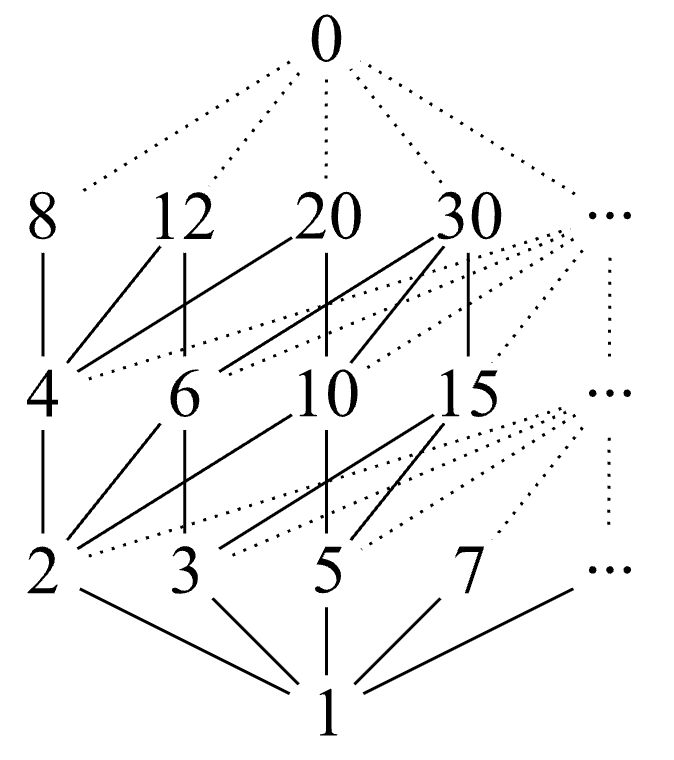
\includegraphics[width=100px]{fig/divisor_lattice.png}
\end{center}

The set $(\mathbb{N}, \preceq)$ forms a preorder. So,
what do products look like in $(\mathbb{N}, \preceq)$ considered 
as a category?
Let's consider the concrete instance of the product of $12$ 
and $16$. Let's consider the three possible interpretations of 
the product of $12$ and $16$ -- let's call it $X$ -- to understand what it means here:\marginnote{In what way 
is this behaving like an intersection?}
\begin{itemize}
  \item The graph-theoretic picture places the product in a diagram. 
  Suppose there is some natural number $Y$ such that $Y \preceq 12$ and $Y \preceq 16$.
  Then, the graphical depiction of the product $X$ 
  asserts the existence of a unique morphism $Y \to X$:
\begin{center}
  % https://tikzcd.yichuanshen.de/#N4Igdg9gJgpgziAXAbVABwnAlgFyxMJZABgBoAmAXVJADcBDAGwFcYkQBGckAX1PUy58hFOQrU6TVuw4A2XvxAZseAkQ6kOEhizaIQADQUCVw9aWLapekAE1eEmFADm8IqABmAJwgBbJADMNDgQSGIgjFhgNlAQODhOxiDefoHBoYhkIABGMGBQSAC0AcR8nj7+iEEgIUgaOXkFVaWKKZXhtZllyRVh6XU8lDxAA
\begin{tikzcd}
  & Y \arrow[d, dotted] \arrow[ldd, bend right] \arrow[rdd, bend left] &    \\
  & X \arrow[ld] \arrow[rd]                                            &    \\
12 &                                                                    & 16
\end{tikzcd}
\end{center}

  \item The order theoretic interpretation tells us that 
  $X$ is the greatest element that is less than both $12$
  and $16$ in the partial order -- i.e., it is the 
  greatest lower bound. In the case of this particular 
  partial order, this object has a special name: it is the 
  greatest common divisor.
\end{itemize}

\section{Initial objects \& duality}
The categorical perspective can push you towards new ideas you may not have
thought of. Here's an example of this: given a category $\calC$, thought of as a
graph, one can do a natural thing: \emph{flip the direction of all arrows in the
opposite direction}. This new category is called the \textbf{opposite category},
and is written $\calC^\text{op}$.
Relationships between properties of $\calC$ and properties of its opposite 
category $\calC^\text{op}$ are broadly referred to as \textbf{dualities}.

Dualities can be a source of free ideas. For instance, let's consider the
dual notion of a terminal object where we flip the direction of the arrows:

\begin{definition}[Initial object] 
  \sloppy
  Let $I$ be an object in a category $\calC$. 
  An object $I$ in $\calC$ is called an initial object
  if, for every other object $A$ in $\calC$ there exists a unique 
  morphism $I \xrightarrow{} C$. Graphically,

  \begin{center}
% https://tikzcd.yichuanshen.de/#N4Igdg9gJgpgziAXAbVABwnAlgFyxMJZABgBpiBdUkANwEMAbAVxiRAEEQBfU9TXfIRQBGclVqMWbACrdxMKAHN4RUADMAThAC2SMiBwQkokAyxhWiEHAhmoIagzoAjGAwAK-PATYMYanAcJZksQAB0wmAAPLDgcOABCOS4gA
\begin{tikzcd}
  I \arrow[r, "\exists!"] & A
  \end{tikzcd}
\end{center}
\end{definition}

Note that an object that is terminal in $\calC$ must be initial 
in $\calC^\text{op}$ and vice versa: this is what characterizes 
the terminal object as dual to the initial object. 

Now that we have a ``free'' universal construction, it might be 
natural to ask: \emph{is there an interesting type that this 
special initial object corresponds to}? Indeed there is: the 
initial object corresponds to the $\plVoid$ type that 
has no inhabitants. It has the following typing rules:

\begin{mathpar}
\inferrule{M : \plVoid}{\Gamma \vdash \texttt{absurd}~M : A}
\end{mathpar}

Intuitively, the $\plVoid$ type represents logical absurdity or 
``invalid program state''.
Some programming languages have a construct for working with 
void types and absurdity: Haskell has the void, which is 
eliminated with \texttt{absurd}.

\section{Products as Terminal Objects ($*$)}
\marginnote{Sections marked with $*$ are optional and won't be covered in class.}

The diagrammatic form suggests a
a order-based intuition for products:
the product \((P,p,q)\) is
in some sense the ``largest''
tuple of that shape,
with its universal property
showing that any other tuple of the same shape is
``less than or equal'' to it by virtue of the existence of
the dashed morphism.

\begin{definition}[category of rooted spans]
  \sloppy
  Let \(A\) and \(B\) be objects of a category \(\calC\).
The category of \emph{spans in \(\calC\) rooted at \(A\) and \(B\)},
written \(\mathsf{Span}_\calC(A,B)\),
is the category whose
\begin{itemize}
  \item Objects are tuples \((X,f,g)\)
    where \(X\) is an object of \(\calC\),
    \(f : X \to A\), and \(g : X \to B\).
    Pictorially:
    \[% https://tikzcd.yichuanshen.de/#N4Igdg9gJgpgziAXAbVABwnAlgFyxMJZABgBoBGAXVJADcBDAGwFcYkQANEAX1PU1z5CKcqWLU6TVuwCCPPiAzY8BIqIBMEhizaIQAIR4SYUAObwioAGYAnCAFskZEDghJ1NbdL2mQNRvQARjCMAAoCKsIgNlimABY48tZ2jojOrkiikjrsVkbcQA
\begin{tikzcd}
                                   & A \\
X \arrow[rd, "g"'] \arrow[ru, "f"] &   \\
                                   & B
\end{tikzcd}\]
  \item A morphism is a tuple
    \(((X,f,g),\alpha,(X',f',g'))\)
    where \((X,f,g)\) and  \((X',f',g')\)
    are objects and \(\alpha : X \to X'\)
    is a morphism of \(\calC\)
    such that \(f' \circ \alpha = f\)
    and \(g' \circ \alpha = g\).
    Pictorially:
    \[% https://tikzcd.yichuanshen.de/#N4Igdg9gJgpgziAXAbVABwnAlgFyxMJZABgBoBGAXVJADcBDAGwFcYkQANEAX1PU1z5CKAEyli1Ok1bsAgjz4gM2PASJiRkhizaIQAIQX8VQouQpbpuzgHIekmFADm8IqABmAJwgBbJGRAcCCQxKR12JxAaRnoAIxhGAAUBVWEQTywnAAscKJB4sCgkAFoAZmJeD28-RACgpHMwmT13PIKixHLKkC9fJFKaesRG7Waeu2i4hOSTNT0M7Nzu3pqBwODEUNHrJztl6v9BjbXt9gAdM6Y0LPp7biA
\begin{tikzcd}
                                                                                &                                       & A \\
X \arrow[rrd, "g"', bend right] \arrow[rru, "f", bend left] \arrow[r, "\alpha"] & X' \arrow[ru, "f'"'] \arrow[rd, "g'"] &   \\
                                                                                &                                       & B
\end{tikzcd}\]

\item Composition is defined by
  \begin{align}
    &((X',f',g'),\alpha',(X'',f'',g''))\circ ((X,f,g),\alpha,(X',f',g'))\\
    &= ((X,f,g),\alpha'\circ \alpha,(X'',f'',g'')).
  \end{align}
  Pictorially:
  \begin{equation}
    % https://tikzcd.yichuanshen.de/#N4Igdg9gJgpgziAXAbVABwnAlgFyxMJZAJgBoAGAXVJADcBDAGwFcYkQBBEAX1PU1z5CKMsWp0mrdgCEefEBmx4CRMgEZxDFm0QgAGgHIDc-kqFE1pDTS1TdhkwoHLhyclc2Sd+493EwoAHN4IlAAMwAnCABbJDIQHAgkdwltdjCjR0iYuJpEpEtUuxBAzJpGegAjGEYABWdzXQisQIALHCyo2MQAZjykxHjbbwAdEaY0VvpfeWzuvoSBlOH04xpqsChk3nCupAX8xEKNrcRlr3ZSkHKqmvqzFSaW9s6cxAAWfuT1mE3987SujCr26n0WBR+f0QAFoegDioFriAKtU6g1HiBmm0OjsQHMkGDDgsVroxhMpjxKNwgA
\begin{tikzcd}
                                                                                 &                                                            & A                                      \\
X' \arrow[rru, "f", bend left] \arrow[rrd, "g"', bend right] \arrow[r, "\alpha"] & X' \arrow[r, "\alpha'"] \arrow[ru, "f'"] \arrow[rd, "g'"'] & X'' \arrow[u, "f''"] \arrow[d, "g''"'] \\
                                                                                 &                                                            & B
\end{tikzcd}
  \end{equation}

  \item The identity morphism at \((X,f,g)\) is \(((X,f,g),\idt_{X},(X,f,g))\).
\end{itemize}
The associativity and identity laws in \(\mathsf{Span}_\calC(A,B)\)
are inherited from the corresponding laws for in \(\calC\).
\end{definition}

This perhaps tortured-looking category serves a valuable purpose:
it makes precise the sense in which a product \((P,p,q)\)
is the ``largest'' among such tuples.

\begin{proposition}
  Let \(A\) and \(B\) be objects of a category \(\calC\).
  A tuple \((P,p,q)\) is a product of \(A\) and \(B\)
  if and only if it is a terminal object of \(\mathsf{Span}_\calC(A,B)\).
\end{proposition}

To unpack what this is saying, from the perspective of categories as metalanguages:
a product for \(A\) and \(B\) in the metalanguage embodied
by \(\calC\) is a unit type for the metalanguage
embodied by \(\mathsf{Span}_\calC(A,B)\).
Some of the power of category theory can be seen here:
\begin{itemize}
\item Constructions on categories can be used to quickly build
  nontrivial ``metalanguages'' from old.
  (What would \(\mathsf{Span}_\calC(A,B)\) even look like as a traditional language?)
\item Category theory ``eats itself'': the categorical notion of terminal object
  sheds light on the categorical notion of product, if one knows to look at
  the right category.
\end{itemize}
To illustrate the benefits of this perspective,
we get a proof that products are suitably unique
just like terminal objects are, simply because they \emph{are terminal objects}:
\begin{proposition}
  Products are unique up to unique isomorphism.
\end{proposition}
\begin{proof}
  Products are terminal objects,
  and terminal objects are unique up to unique isomorphism.
\end{proof}



\chapter{Universal Constructions II}

Let us recall the rules for a language with function types.
First, we have the rule for making terms of function type:
\begin{mathpar}
\inferrule*
    {\Gamma, x \ofty A \vdash M : B}
    {\Gamma \vdash \pllam{x}{M} : A \plto B}
    ~(\textsc{T-Lam})
\end{mathpar}
Next, we have the elimination rule for using terms of function type:
\begin{mathpar}
\inferrule*
    {\Gamma\vdash M : A \plto B
      \\
    \Gamma \vdash N : A
    }
    {\Gamma \vdash \plapp{M}{N} : B}
    ~(\textsc{T-App})
\end{mathpar}
Finally, we have the \(\beta\) and \(\eta\) laws,
which state that applying a function corresponds to
substitution and that every term of function type is equivalent
to a \(\lambda\)-expression.
\begin{mathpar}
\inferrule*
    {
      \Gamma, x\ofty A\vdash M : B
      \\
      \Gamma \vdash N : A
    }
    {\Gamma \vdash \plapp{(\pllam{x}{M})}{N} \equiv M[N/x] : B}
    ~(\beta^{\plto})
\and
\inferrule*
    {\Gamma \vdash M : A \to B}
    {\Gamma \vdash M \equiv \pllam{x}{\plapp{M}{x}} : A \to B}
    ~(\eta^{\plto})
\end{mathpar}

In category theory, this language feature is captured by
the concept of an \emph{exponential object}.
\newcommand\app{\mathsf{app}}
\newcommand\lam{\lambda}
\begin{definition} \label{def:exponential}
  \sloppy
  Let \(A\) and \(B\) be objects of a category \(\calC\) with products.
  An \emph{exponential of \(A\) by \(B\)}
  is a pair \((E,\app)\) consisting of
  an object \(E\) of \(\calC\)
  and a morphism
  \(\app : E\times A \to B\)
  such that the following universal property holds:
  for all morphisms \(f : \Gamma \times A \to B\),
  there exists a unique morphism \(\lam f : \Gamma \to E\)
  such that \(\app \circ \angled{\lam f \circ \pi_1, \pi_2} = f\).
\end{definition}

Note that the morphism \(\app\)
has a domain defined by a product,
and the universal property of \((E,\app)\)
is stated in terms of the morphism \(\angled{\lam f \circ \pi_1,\pi_2}\),
whose existence depends on the existence of products.
So the definition of exponential objects
requires products in \(\calC\) as a prerequisite.%
\footnote{There are actually tricks to define
the notion of ``function object'' categorically
without reference to products, but that will have to wait until after Yoneda IV.}

\noindent How does this definition capture the familiar rules for function types?
\begin{itemize}
  \item The object \(E\) models the function space \(A \to B\).
  \item \(\app\) corresponds to function application:
    \(f\ofty E, a\ofty A \vdash f\plapp a : B\).
  \item The universal property models \textsc{T-Lam}.
  \item What to make of the equation \(\app \circ \angled{\lam f \circ \pi_1, \pi_2} = f\)?
\end{itemize}

\noindent To understand, we need to take a slightly more detailed look at how to
    translate terms into categorical combinators.
\begin{itemize}
  \item Recap of products: each term formation rule becomes an operation on morphisms.
    Typing derivations can be translated into categorical combinators this way.
    Example: fst (a, b)
  \item Each equational law becomes an equality of composites.
    Example: fst (a, b) = a.
  \item Subtle point: weakening as precomposition by structural maps.
    Example: suppose M is well typed under Gamma; interpret M under Gamma,a:A.
\end{itemize}
\begin{align*}
  \inferrule*[right=T-Wk]
    {\Gamma \vdash M : B}
    {\Gamma, a\ofty A \vdash M : B}
  \qquad\raisebox{1em}{\(\leadsto\)}\qquad
  \inferrule*[right=C-Wk]
    {\Gamma \xlongrightarrow{f} B}
    {\Gamma \times A \xlongrightarrow{f\,\circ\,\pi_1} B}
\end{align*}
Note that we are blurring the distinction between syntactic and mathematical objects here:
in the rule on the left, \(\Gamma\) is a typing context, \(A\) and \(B\)
are syntactic types, and \(M\) is a term;
in the rule on the right, \(\Gamma\), \(A\), and \(B\) are all objects of an
arbitrary category \(\calC\) with products,
and \(f\) an arbitrary morphism \(\Gamma \to B\).

The universal property of
Definition~\ref{def:exponential}
provides a categorical analog of the typing rules \textsc{T-Lam}:
\begin{align*}
  \inferrule*[right=T-Lam]
    {\Gamma, a\ofty A \vdash M : B}
    {\Gamma \vdash \pllam{a}{M} : A \plto B}
  \qquad&\raisebox{1em}{\(\leadsto\)}\qquad
  \inferrule*[right=C-Lam]
    {\Gamma \times A \xlongrightarrow{f} B}
    {\Gamma \xlongrightarrow{\lam f} E}
\end{align*}
The morphism \(\app\) can be used to construct a categorical analog of \textsc{T-App}:
\begin{align*}
  \inferrule*[right=T-App]
    {
      \Gamma \vdash M : A \plto B
      \\\\
      \Gamma \vdash N : A
    }
    {\Gamma \vdash \plapp{M}{N} : B}
  \qquad&\raisebox{1em}{\(\leadsto\)}\qquad
  \inferrule*[right=C-App]
    {
      \Gamma \xlongrightarrow{f} E
      \\\\
      \Gamma \xlongrightarrow{g} A
    }
    {\Gamma \xlongrightarrow{\app\,\circ\,\angled{f,g}} B}
\end{align*}
The rule on the right skips a few steps
in order to make its shape fit that of the standard typing rule
for function application: the morphism displayed in its conclusion
tree is built by first using the universal property of the product \(E\times A\)
to form the tupling \(\angled{f,g}\) of the morphisms in its premises,
and then composing with \(\app\).
You can think of this rule as an abbreviation for a
more detailed proof tree:
\begin{mathpar}
  \inferrule*
    {
      \inferrule*
        {
          \Gamma\xlongrightarrow{f} E
          \\
          \Gamma\xlongrightarrow{g} A
        }
        {\Gamma\xlongrightarrow{\angled{f,g}} E \times A}
      \\
      \inferrule*{~}{E \times A \xlongrightarrow{\app} B}
    }
    {\Gamma \xlongrightarrow{\app\,\circ\,\angled{f,g}} B}
\end{mathpar}

There still remains the question of how to interpret the side condition
accompanying the universal property: namely, that \(\lam f\)
is the unique solution to the equation
\(\app \circ \angled{\lam f \circ \pi_1, \pi_2} = f\).

As a first step to understanding this condition, let us first translate
the equation \(\app \circ \angled{\lam f \circ \pi_1, \pi_2} = f\)
into familiar language.
The following ``typing derivation'' shows how
the left-hand side of this equation can be built up
from its components:
\begin{mathpar}
  \inferrule*[right=C-App]
    {
      \inferrule*[right=C-Wk]
        {
          \inferrule*[right=C-Lam]
            {\Gamma \times A \xlongrightarrow{f} B}
            {\Gamma \xlongrightarrow{\lam f} E}
        }
        {\Gamma \times A \xlongrightarrow{\lam f \circ \pi_1} E}
      \\
      \inferrule*[right=C-Var]{~}{\Gamma \times A \xlongrightarrow{\pi_2} A}
    }
    {\Gamma \times A \xlongrightarrow{\app\,\circ\,\angled{\lam f \circ \pi_1, \pi_2}} B}
\end{mathpar}
Reading this tree from the top down:
first, the morphism \(f\)
is turned into a morphism
\(\lam f\) by the universal property of \((E,\app)\),
and composed with the projection \(\pi_1\)
to yield the composite \(\Gamma\times A \xrightarrow{\lam f \circ \pi_1} E\).
This composite is then tupled with \(\Gamma \times A \xrightarrow{\pi_2} A\)
using the universal property of the product \(E\times A\)
to form \(\Gamma\times A \xrightarrow{\angled{\lam f \circ \pi_1,\pi_2}} E \times A\),
and then composed with \(\app\)
to form the morphism shown at the root.

This ``meta-level derivation''
can be translated back into an object language one
by replacing each use of a categorical typing rule
with its syntactic counterpart:
\begin{mathpar}
  \inferrule*[right=T-App]
    {
      \inferrule*[right=T-Wk]
        {
          \inferrule*[right=T-Lam]
            {\Gamma, a\ofty A \vdash M : B}
            {\Gamma \vdash \pllam{a}{M} : A \plto B}
        }
        {\Gamma, a\ofty A \vdash \pllam{a}{M} : A \plto B}
      \\
      \inferrule*[right=T-Var]{~}{\Gamma, a\ofty A \vdash a : A}
    }
    {\Gamma, a \ofty A \vdash \plapp{(\pllam{a}{M})}{a} : B}
\end{mathpar}

Now let us reexamine the universal property of exponentials,
which says that
for each \(f\) there is a unique \(\lam f\)
such that \(\app \circ \angled{\lam f \circ \pi_1, \pi_2} = f\).
There are two parts to this assertion:
\begin{enumerate}
\item (Existence) There is a morphism, called \(\lam f\),
  such that \(\app \circ \angled{\lam f \circ \pi_1, \pi_2} = f\).
\item (Uniqueness) If \(g\) is a morphism
  such that \(\app \circ \angled{g \circ \pi_1, \pi_2} = f\),
  then it must be the case that \(g = \lam f\).
\end{enumerate}

Existence corresponds to the following equation between terms:
\begin{mathpar}
  \inferrule*
    {\todo}
    {\Gamma, a \ofty A \vdash \plapp{(\pllam{a}{M})}{a} \equiv M : B}
\end{mathpar}
This equation has an intuitive reading: it is a special case
of \(\beta^{\plto}\), where the argument to \(\pllam{a}{M}\)
is a single variable.
Note something a little magical is happening here:
the two occurrences of \(M\) in this equation have different
binding structure. On the left-hand side, occurrences of \(a\)
in \(M\) refer to the bound variable in \(\pllam{a}{M}\),
whereas on the right-hand side they refer to the binding \(a\ofty A\)
in the typing context.

Uniqueness says that if \(\Gamma \vdash M : A \plto B\) is any
term such that \(\Gamma, a \ofty A \vdash \plapp{M}{a} \equiv N : B\),
then \(\Gamma \vdash M \equiv \pllam{a}{N} : A \plto B\).
As a proof rule,
\begin{mathpar}
  \inferrule*
    {
      \Gamma, a \ofty A \vdash \plapp{M}{a} \equiv N : B
    }
    {\Gamma \vdash M \equiv \pllam{a}{N} : A \plto B}
\end{mathpar}
This rule is interderivable with \(\eta^{\plto}\).




\begin{itemize}
  \item Recall the three perspectives:
    \begin{itemize}
    \item Algebraic: beta and eta rules as equations
    \item Graphical: the triangle commutes
    \item Order-theoretic: exponential as largest code pointer (formally:
            terminal in a category of code pointers)
    \end{itemize}
\end{itemize}
\todo

\begin{itemize}
  \item Examples
    \begin{itemize}
    \item Exponentials in FinSet are function spaces
    \item Exponentials in open subsets of the plane are a funny thing (remember:
      largest code pointer)
    \end{itemize}
\end{itemize}
\todo

\section{Getting formal about categorical semantics}

\begin{itemize}
  \item What's really going on?
\end{itemize}
Wellformedness rules
\[
s ::= (M,\dots)
\]
\[
\fbox{\(s : \Gamma \longrightarrow \Gamma'\)}
\]
\begin{mathpar}
\inferrule
    {\Gamma \vdash M : A
      \\\dots}
    {(M,\dots) : \Gamma \longrightarrow x\ofty A,\dots}
\end{mathpar}
The following rule is admissible:
\begin{mathpar}
  \inferrule{\Gamma \vdash M : A \\ s : \Gamma'\longrightarrow\Gamma}
            {\Gamma' \vdash M[s] : A}
\end{mathpar}
Semantically,
\[
\text{if \(s : \Gamma\longrightarrow\Gamma'\)
then \(\llbr{s} : \llbr{\Gamma} \to \llbr{\Gamma'}\)}
\]
\footnote{The dreaded ``substitution lemma'' that all mechanizers hate}
\[
\llbr{M[s]} = \llbr{M} \circ \llbr{s}
\]
All semantic interpretation functions must be stable
under substitution/precomposition:
\begin{align*}
  \plpair{M}{N}[s] &= \plpair{M[s]}{N[s]}
  &
  \angled{f,g} \circ p &= \angled{f\circ p,g\circ p}
  \\
  \plfst{M}[s] &= \plfst{M[s]}
  &
  (\pi_1 \circ f) \circ p &= \pi_1 \circ (f \circ p)
\end{align*}

\begin{itemize}
  \item Distributivity, ``high school algebra laws''
\end{itemize}
\todo

%%%%%%%%%%%%%%%%%%%%%%%%%%%%%%%%%%%%%%%%%%%%%%%%%%%%%%%%%%%%%%%%%%%%%%%%%%%%%%%%
%%%%%%%%%%%%%%%%%%%%%%%%%%%%%%%%%%%%%%%%%%%%%%%%%%%%%%%%%%%%%%%%%%%%%%%%%%%%%%%%


% - Give standard rules for function types
% - Golf rules using substitution
% - Reverse engineer textbook definition


\chapter{Yoneda I}

\noindent In set theory, functions enjoy the following nice properties.
\begin{enumerate}
\item Extensional equality: two functions \(f,g : X \to Y\)
  are equal if and only if \(f(x) = g(x)\) for all elements \(x\) of \(X\).
\item Elementwise definition:
  to define a function \(f : X \to Y\),
  it suffices give a relation,
  called the \emph{graph of \(f\)},
  such that each element \(X\)
  is related exactly one element of \(Y\).
\end{enumerate}
The presence of elements makes functions much easier to work with.
For instance, compare the proof \(X \times (Y \times Z) \cong (X\times Y) \times Z\)
as sets with the abstract proof for an arbitrary category with products.

In this chapter we will see how to recover a similar kind of element-wise reasoning
style that works in an arbitrary category.
While objects of categories don't have elements,
they do have \emph{generalized elements},
which bring much of the benefits of elements in set theory
to working in arbitrary categories.

The starting point for this generalization is the following
proposition, which recasts ``element of a (finite) set'' into categorical language.
\begin{proposition}[Elements in \(\FinSet\)]
  Let \(X\) be an object of \(\FinSet\).
  Elements of \(X\) are in bijection
  with morphisms of \(\FinSet\)
  from \(1\) to \(X\).
\end{proposition}
In light of this proposition, properties (1) and (2)
above translate into the following statements about \(\FinSet\):
\begin{itemize}
\item \textbf{(Property 1)} Extensional equality:
  Two morphisms \(f,g : X \to Y\)
  in \(\FinSet\) are equal if and only if \(f \circ x = g \circ x\)
  for all morphisms \(x : 1 \to X\).
\item \textbf{(Property 2)} Elementwise definition:
  to define a morphism \(f : X \to Y\)
  of \(\FinSet\),
  it suffices to give a relation \(R\)
  such that each
  morphism \(1 \to X\)
  is related to exactly one morphism \(1 \to Y\).
\end{itemize}

\sh{Let's slow down and give some concrete examples of 
``reasoning pointwise'' in finset. Give an example of 
this element-wise definition.}

\sh{define the notion of ``testing'' objects in a 
category by considering morphisms into them}

\section{From sets to categories}
\sh{Transition systems, canonical loop and canonical edge}

How to generalize the above situation to an arbitrary category?
An arbitrary category might not have a terminal object \(1\).
Even if they do, it's not guaranteed that functions can be
defined and tested for equality simply via morphisms \(1 \to X\).

The trick is to replace the special object \(1\)
with a \emph{quantification over all possible objects}.
Compare the statement of extensionality for \(\FinSet\)
above with the following proposition, which holds in any category:

\begin{proposition}[Generalized extensionality] \label{prop:generalized-extensionality}
  Let \(f,g : X \to Y\) be two morphisms in a category \(\calC\).
  Suppose that \(f \circ x = g \circ x\) for all objects \(\Gamma\)
  and all morphisms \(x : \Gamma \to X\).
  Then \(f = g\).
\end{proposition}
\begin{proof}
  Letting \(\Gamma = X\) and \(x = \idt_X\) gives \(f \circ \idt_X = g \circ \idt_X\).
  Simplifying yields \(f = g\).
\end{proof}

\begin{definition}[Generalized element]
  Let \(X\) and \(\Gamma\) be objects of a category \(\calC\).
  A \emph{generalized element of \(X\) at stage \(\Gamma\)}
  is a morphism \(x : \Gamma \to X\).
  The set of generalized elements of \(X\) at stage \(\Gamma\)
  will be written \(\genelt{X}{\Gamma}\).
\end{definition}

In this new language, Proposition~\ref{prop:generalized-extensionality}
says that two morphisms of a category are equal if
they act the same on all generalized elements.

Generalizing the principle of property 2, the elementwise definition,
is trickier. Since the single object \(1\) has been replaced by a quantification over
all objects \(\Gamma\), the notion of ``function'' as graph
needs to be adjusted similarly.

\begin{definition}[Generalized function]
  Let \(X,Y\) be objects of a category \(\calC\).
  A \emph{generalized function} \(\varphi\) from \(X\) to \(Y\)
  is a family of functions
  \(\varphi_\Gamma \subseteq \genelt{X}{\Gamma} \to \genelt{Y}{\Gamma}\)
  indexed by objects \(\Gamma\) of \(\calC\)
  that respects ``change of stage''
  in the sense that for all \(p : \Gamma' \to \Gamma\)
  and all \(x \in \genelt{X}{\Gamma}\)
  it holds that \(\varphi_\Gamma(x\circ p) = \varphi_\gamma(x)\circ p\).
\end{definition}

\begin{proposition}[Generalized elementwise definition]
  \label{prop:generalized-elementwise-definition}
  Let \(X,Y\) be objects of a category \(\calC\).
  Let \(\varphi\) be a generalized function from \(X\) to \(Y\).
  There exists a morphism \(f : X \to Y\)
  such that \(\varphi_\Gamma(x) = f \circ x\)
  for all objects \(\Gamma\) and all \(x \in \genelt{X}{\Gamma}\).
\end{proposition}

\begin{proposition}
  \(X \times (Y\times Z) \cong (X \times Y) \times Z\)
  in any category \(\calC\) with products.
\end{proposition}
\begin{proof}
  Let \(\varphi\) be a family of functions
  from generalized elements of \(X \times (Y\times Z)\)
  to generalized elements of \((X\times Y) \times Z\)
  defined as follows:
  \[
  \varphi_\Gamma\angled{x,\angled{y,z}}
  =\angled{\angled{x,y},z}
  \text{ for all \(x:\Gamma\to X,y:\Gamma\to Y,z:\Gamma\to Z\)}
  \]
  This function respects change of stage:
  \begin{align}
    \varphi_\Gamma\angled{x,\angled{y,z}}\circ p
    &= \angled{\angled{x,y},z}\circ p\\
    &= \angled{\angled{x\circ p,y\circ p},z \circ p}\\
    &= \varphi_\Gamma\angled{x\circ p,\angled{y\circ p,z\circ p}}\\
    &= \varphi_\Gamma(\angled{x,\angled{y,z}}\circ p).
  \end{align}
  Hence \(\varphi\) is a generalized function from \(X \times (Y\times Z)\)
  to \((X\times Y) \times Z\) and,
  by generalized elementwise definition,
  there exists a morphism \(f : X \times (Y\times Z) \to (X\times Y) \times Z\),
  such that \(f\circ \angled{x,\angled{y,z}}
  = \varphi_\Gamma\angled{x,\angled{y,z}}
  = \angled{\angled{x,y},z}\)
  for all objects \(\Gamma\) and morphisms \(x:\Gamma\to X,y:\Gamma\to Y,z:\Gamma\to Z\).

  Similarly, we can define a morphism \(g\) going the other way,
  in terms of the following generalized function \(\psi\):
  \[
  \psi_\Gamma\angled{\angled{x,y},z} = \angled{x,\angled{y,z}}.
  \]

  Now for
  all objects \(\Gamma\) and morphisms \(x:\Gamma\to X,y:\Gamma\to Y,z:\Gamma\to Z\),
  it holds that
  \begin{align}
    (f\circ g)\circ \angled{\angled{x,y},z}
    &= f\circ (g\circ \angled{\angled{x,y},z}) \\
    &= f\circ (\psi_\Gamma\angled{\angled{x,y},z}) \\
    &= f\circ \angled{x,\angled{y,z}} \\
    &= \varphi_\Gamma\angled{x,\angled{y,z}} \\
    &= \angled{\angled{x,y},z} \\
    &= \idt_{(X\times Y) \times Z} \circ \angled{\angled{x,y},z}
  \end{align}
  so \(f\circ g = \idt_{(X\times Y) \times Z}\)
  by generalized extensionality.

  An analogous argument gives \(g \circ f = \idt_{X\times (Y\times Z)}\).
  Hence \(f\) and \(g\) form an isomorphism
  between \(X \times (Y\times Z)\) and \((X\times Y) \times Z\).
\end{proof}
Note the similarity between this proof and the standard set-theoretic
argument that \(X \times (Y\times Z) \cong (X \times Y) \times Z\)
when \(X,Y,Z\) are sets.
The key differences in this more general setting are (1)
the quantification over stages \(\Gamma\)
and (2) the checks that generalized functions respect change of stage.

If you want to learn more about this perspective, check out
Tom Leinster's ``\href{https://webhomes.maths.ed.ac.uk/~tl/elements.pdf}{Doing without diagrams}''.

\chapter{Yoneda II: indexed set theory and representability}

Throughout this section we will work with an arbitrary catetgory \(\calC\).

\begin{definition}
  A \emph{\(\calC\)-indexed set}
  consists of a family of sets \(PX\) indexed by objects \(X\) of \(\calC\),
  along with ``substitution functions'' \(Pf : PY \to PX\)
  for each morphism \(f : X \to Y\) in \(C\).
  Given an element \(y \in PY\)
  and a morphism \(f : X \to Y\),
  the element \((Pf)(y)\) will be written \(y \cdot_P f\)
  and called the ``substitution of \(y\) by \(f\)''.
  Every \(\calC\)-indexed set \(P\)
  must satisfy the following laws:
  \begin{itemize}
  \item Identity: \(x \cdot_P \idt_X = x\) for all objects \(X\) and \(x \in PX\)
  \item Composition: \(z \cdot_P (f\circ g) = z \cdot_P f \cdot_P g\)
    for all objects \(f : Y \to Z\) and \(g : X \to Y\) and \(z \in PZ\).
  \end{itemize}
\end{definition}

\begin{example}
  Recall that \(\mathsf{STLC}\) is a category
  whose objects are types and whose morphisms \(A \to B\)
  are terms \(x : A \vdash M : B\) quotiented by \(\beta\eta\)-equivalence.
  For each type \(A\),
  the following defines a \(\mathsf{STLC}\)-indexed set \(\mathsf{Tm}(A)\):
  \begin{align}
  \mathsf{Tm}(B)(A) &= \text{the set of morphisms \(A\to B\)} \\
  \mathsf{Tm}(B)(N : A'\to A)
  &= (x\ofty A \vdash M : B) \mapsto (x'\ofty A' \vdash M[N/x] : B)
  \end{align}
\end{example}
This example is a special case of a canonical kind of \(\calC\)-indexed set.
\begin{definition}
  The \emph{representable \(\calC\)-indexed set at \(X\)}
  is written \(\yo X\) and defined by
  \begin{align}
    (\yo X)(A) &= \text{the set of morphisms \(A \to X\)} \\
    (\yo X)(A)(s : A' \to A) &= (f : A \to X) \mapsto (f \circ s : A' \to X)
  \end{align}
\end{definition}

\begin{definition}
  \sloppy
  Let \(P\) and \(Q\) be \(\calC\)-indexed sets.
  A \emph{\(\calC\)-indexed function}
  from \(P\) to \(Q\),
  written \(\alpha : P \Rightarrow Q\),
  is a family of functions \(\alpha_X : PX \to QX\)
  that ``respects substitution''
  in the sense that \(\alpha_{X'}(x\cdot_P p) = \alpha_X(x)\cdot_p p\).
\end{definition}

\begin{itemize}
\item \(\calC\)-indexed functions can be composed:
  the composition of \(\alpha : Q \Rightarrow R\)
  and \(\beta: P \Rightarrow Q\),
  written \(\alpha\circ\beta : P \Rightarrow R\),
  is defined by \((\alpha\circ\beta)_X = \alpha_X \circ \beta_X\).
\item For each \(\calC\)-indexed set \(P\),
  there is a \(\calC\)-indexed function \(\idt_P : P \Rightarrow P\)
  defined by \(\idt_{P,X} = \left(PX \xrightarrow{\idt_{PX}} PX\right)\).
\end{itemize}
By now you may have noticed that \(\calC\)-indexed sets and functions
look like they ought to form a category. More on this later.

\begin{definition}
  Two \(\calC\)-indexed sets \(P,Q\)
  are \emph{isomorphic}
if there are \(\calC\)-indexed functions \(\alpha : P \Rightarrow Q\)
and \(\beta : Q \Rightarrow P\)
such that \(\alpha\circ\beta=\idt_Q\) and \(\beta\circ\alpha=\idt_P\).
\end{definition}

\begin{definition}
  A \(\calC\)-indexed set \(P\) is \emph{representable}
  if there is an isomorphism \(\alpha : P \cong \yo X : \beta\)
  for some object \(X\) of \(\calC\).
\end{definition}

\chapter{Yoneda III: universal constructions, elements, and properties}

\begin{definition}
  \sloppy
  Given two \(\calC\)-indexed sets \(P\) and \(Q\),
  their \emph{product} \(P\times Q\)
  is the \(\calC\)-indexed set defined by
  \((P\times Q)(X) = P(X)\times Q(X)\),
  with substitution defined by
  \((x,y)\cdot_{P\times Q} p = (x\cdot_P p, y\cdot_Q p)\).
\end{definition}

\begin{proposition}
  Let \(X\) and \(Y\) be two objects of a category \(\calC\).
  An object \(P\) is a product of \(X\) and \(Y\)
  if and only if \(\yo P\) is isomorphic to \(\yo X \times \yo Y\).
\end{proposition}

\begin{definition}
  Given two objects \(X\) and \(Y\) of a category \(\calC\),
  there is a \(\calC\)-indexed set of \emph{closures},
  written \(\mathsf{Clos}(X,Y)\),
  defined by \(\mathsf{Clos}(X,Y)(\Gamma) = \calC(\Gamma\times X, Y)\),
  with substitution defined by
  \[
    \mathsf{Clos}(X,Y)(s : \Gamma'\to \Gamma)(f : \Gamma\times X \to Y)
    = \angled{\gamma',x} \mapsto f \circ \angled{s\circ \gamma', x}
  \]
  on generalized elements.
\end{definition}

\begin{proposition}
  Let \(X\) and \(Y\) be two objects of a category \(\calC\).
  An object \(E\) is the exponential \(Y^X\)
  if and only if \(\yo E\) is isomorphic to \(\mathsf{Clos}(X,Y)\).
\end{proposition}

\begin{proposition}
  Suppose the \(\calC\)-indexed set \(P\) is represented
  by the object \(X\).
  Then there exists an element \(u \in PX\),
  called the \emph{\(P\)-universal element},
  which satisfies the following \emph{universal property}:
  for any object \(\Gamma\) and any element \(g \in P\Gamma\),
  there exists a unique morphism \(\hat g : \Gamma \to X\)
  such that \(g = u \cdot_P \hat g\).
\end{proposition}

\begin{itemize}
\item In the case of the product, with \(\yo P \cong \yo X \times \yo Y\),
  the universal element is an element \(u \in \calC(P,X) \times \calC(P,Y)\),
  which is a pair of morphisms \(P\to X, P\to Y\).
  The universal property of this pair is that any other pair \(\Gamma \to X,\Gamma\to Y\)
  factors uniquely through it---precisely the universal property of products
\item In the case of exponents, with \(\yo E \cong \calC(A\times(-),B)\),
  the universal element is an element \(u \in \calC(A \times E,B)\),
  which is a morphism \(A \times E \to B\).
  The universal property of this morphism is that any other morphism
  \(A \times \Gamma \to B\)
  factors uniquely through it---precisely the universal property of exponents.
\end{itemize}

\chapter{Yoneda IV}

%% - Grothendieck universes
%% - The category Set
%% - Functors; opposite categories; C-indexed sets as functors
%% - Natural transformations; C-indexed functions as natural transformations
%% - The Yoneda lemma (without showing naturality in P,c)

%% \begin{itemize}
%% \item Functors form a category where morphisms are natural transformations \begin{itemize}
%%     \item Natural transformations as homotopies between diagrams
%%       (the \(C\to D^\to\) example revisited)
%%     \item Natural transformations as polymorphic maps
%%   \end{itemize}
%% \item Definition of Yoneda embedding
%% \item Restatement of universal properties from previous week in terms of Yoneda embedding
%% (e.g., for products, \(\yo(a\times b) \cong \yo(a)\times \yo(b)\).)
%% \item Yoneda embedding full and faithful. Use this to quickly prove some basic facts:
%%   associativity and commutativity of sums and products, distributivity of products over sums,
%%   ...
%%   These imply type isomorphisms in STLC and Set, entailments of propositional logic.
%% \item Yoneda preserves limits.
%%   This gives a quick proof that all limits can be constructed from products and equalizers.
%%   From this we can compute limits in STLC (it won't have all of them
%%   but it will have some).
%% \end{itemize}

%% \todo: \begin{itemize}
%% \item Slice over c is category of elements of yo c
%% \end{itemize}

\chapter{Week 3: adjoints}

\begin{itemize}
\item We've seen three examples of ``inverses to product'':
  exponentiation in STLC, magic wand in separation logic,
  and lollipop in linear type theory.
  These are all instances of adjunctions.
\item Adjoints as a whole family of universal properties (recast univ. prop. of
  (co)products, pullbacks, (co)limits more generally in these terms)
\item Adjoints as approximate inverses (Galois connections in AI, comma category
  statement. Example: biorthogonal closure)
\item Right adjoints preserve limits, and left adjoints preserve colimits.
    This immediately shows \begin{itemize}
      \item In STLC, $\times$ distributes over $+$
      \item Separating conjunction distributes over disjunction
      \item Magic wand distributes over conjunction
    \end{itemize}
\item Adjoints are unique up to unique isomorphism. Application:
  calculate exponents of presheaves
\item Fun reference: \href{https://golem.ph.utexas.edu/category/2025/02/universal_characterization_of.html#c063905}{Meas is not cartesian closed}
\end{itemize}


\bibliographystyle{plain}
\bibliography{lib/bib}

\end{document}
